\documentclass[12pt,twoside]{article}

\newcommand{\reporttitle}{495 Advanced Statistical Machine Learning and Pattern Recognition}
\newcommand{\reportauthor}{Thomas Teh}
\newcommand{\reporttype}{Notes}
\newcommand{\cid}{0124 3008}

% include files that load packages and define macros
%%%%%%%%%%%%%%%%%%%%%%%%%%%%%%%%%%%%%%%%%
% University Assignment Title Page 
% LaTeX Template
% Version 1.0 (27/12/12)
%
% This template has been downloaded from:
% http://www.LaTeXTemplates.com
%
% Original author:
% WikiBooks (http://en.wikibooks.org/wiki/LaTeX/Title_Creation)
%
% License:
% CC BY-NC-SA 3.0 (http://creativecommons.org/licenses/by-nc-sa/3.0/)
% 
% Instructions for using this template:
% This title page is capable of being compiled as is. This is not useful for 
% including it in another document. To do this, you have two options: 
%
% 1) Copy/paste everything between \begin{document} and \end{document} 
% starting at \begin{titlepage} and paste this into another LaTeX file where you 
% want your title page.
% OR
% 2) Remove everything outside the \begin{titlepage} and \end{titlepage} and 
% move this file to the same directory as the LaTeX file you wish to add it to. 
% Then add \input{./title_page_1.tex} to your LaTeX file where you want your
% title page.
%
%----------------------------------------------------------------------------------------
%	PACKAGES AND OTHER DOCUMENT CONFIGURATIONS
%----------------------------------------------------------------------------------------
\usepackage{ifxetex}
\usepackage{textpos}
\usepackage{natbib}
%\usepackage{breqn}
\usepackage{kpfonts}
\usepackage[a4paper,hmargin=2.8cm,vmargin=2.0cm,includeheadfoot]{geometry}
\usepackage{ifxetex}
\usepackage{stackengine}
\usepackage{tabularx,longtable,multirow,subfigure,caption}%hangcaption
\usepackage{fncylab} %formatting of labels
\usepackage{fancyhdr}
\usepackage{color}
\usepackage[tight,ugly]{units}
\usepackage{url}
\usepackage{float}
\usepackage[english]{babel}
\usepackage{amsmath}
\usepackage{graphicx}
\usepackage[colorinlistoftodos]{todonotes}
\usepackage{dsfont}
\usepackage{epstopdf} % automatically replace .eps with .pdf in graphics
\usepackage{natbib}
\usepackage{backref}
\usepackage{array}
\usepackage{latexsym}
\usepackage{etoolbox}

\usepackage{enumerate} % for numbering with [a)] format 



\ifxetex
\usepackage{fontspec}
\setmainfont[Scale=.8]{OpenDyslexic-Regular}
\else
\usepackage[pdftex,pagebackref,hypertexnames=false,colorlinks]{hyperref} % provide links in pdf
\hypersetup{pdftitle={},
  pdfsubject={}, 
  pdfauthor={\reportauthor},
  pdfkeywords={}, 
  pdfstartview=FitH,
  pdfpagemode={UseOutlines},% None, FullScreen, UseOutlines
  bookmarksnumbered=true, bookmarksopen=true, colorlinks,
    citecolor=black,%
    filecolor=black,%
    linkcolor=black,%
    urlcolor=black}
\usepackage[all]{hypcap}
\fi

\usepackage{tcolorbox}

% various theorems
\usepackage{ntheorem}
\theoremstyle{break}
\newtheorem{lemma}{Lemma}
\newtheorem{theorem}{Theorem}
\newtheorem{remark}{Remark}
\newtheorem{definition}{Definition}
\newtheorem{proof}{Proof}

% example-environment
\newenvironment{example}[1][]
{ 
\vspace{4mm}
\noindent\makebox[\linewidth]{\rule{\hsize}{1.5pt}}
\textbf{Example #1}\\
}
{ 
\noindent\newline\makebox[\linewidth]{\rule{\hsize}{1.0pt}}
}



%\renewcommand{\rmdefault}{pplx} % Palatino
% \renewcommand{\rmdefault}{put} % Utopia

\ifxetex
\else
\renewcommand*{\rmdefault}{bch} % Charter
\renewcommand*{\ttdefault}{cmtt} % Computer Modern Typewriter
%\renewcommand*{\rmdefault}{phv} % Helvetica
%\renewcommand*{\rmdefault}{iwona} % Avant Garde
\fi

\setlength{\parindent}{0em}  % indentation of paragraph

\setlength{\headheight}{14.5pt}
\pagestyle{fancy}
\fancyfoot[ER,OL]{\thepage}%Page no. in the left on
                                %odd pages and on right on even pages
\fancyfoot[OC,EC]{\sffamily }
\renewcommand{\headrulewidth}{0.1pt}
\renewcommand{\footrulewidth}{0.1pt}
\captionsetup{margin=10pt,font=small,labelfont=bf}


%--- chapter heading

\def\@makechapterhead#1{%
  \vspace*{10\p@}%
  {\parindent \z@ \raggedright %\sffamily
        %{\Large \MakeUppercase{\@chapapp} \space \thechapter}
        %\\
        %\hrulefill
        %\par\nobreak
        %\vskip 10\p@
    \interlinepenalty\@M
    \Huge \bfseries 
    \thechapter \space\space #1\par\nobreak
    \vskip 30\p@
  }}

%---chapter heading for \chapter*  
\def\@makeschapterhead#1{%
  \vspace*{10\p@}%
  {\parindent \z@ \raggedright
    \sffamily
    \interlinepenalty\@M
    \Huge \bfseries  
    #1\par\nobreak
    \vskip 30\p@
  }}
  



% %%%%%%%%%%%%% boxit
\def\Beginboxit
   {\par
    \vbox\bgroup
	   \hrule
	   \hbox\bgroup
		  \vrule \kern1.2pt %
		  \vbox\bgroup\kern1.2pt
   }

\def\Endboxit{%
			      \kern1.2pt
		       \egroup
		  \kern1.2pt\vrule
		\egroup
	   \hrule
	 \egroup
   }	

\newenvironment{boxit}{\Beginboxit}{\Endboxit}
\newenvironment{boxit*}{\Beginboxit\hbox to\hsize{}}{\Endboxit}



\allowdisplaybreaks

\makeatletter
\newcounter{elimination@steps}
\newcolumntype{R}[1]{>{\raggedleft\arraybackslash$}p{#1}<{$}}
\def\elimination@num@rights{}
\def\elimination@num@variables{}
\def\elimination@col@width{}
\newenvironment{elimination}[4][0]
{
    \setcounter{elimination@steps}{0}
    \def\elimination@num@rights{#1}
    \def\elimination@num@variables{#2}
    \def\elimination@col@width{#3}
    \renewcommand{\arraystretch}{#4}
    \start@align\@ne\st@rredtrue\m@ne
}
{
    \endalign
    \ignorespacesafterend
}
\newcommand{\eliminationstep}[2]
{
    \ifnum\value{elimination@steps}>0\leadsto\quad\fi
    \left[
        \ifnum\elimination@num@rights>0
            \begin{array}
            {@{}*{\elimination@num@variables}{R{\elimination@col@width}}
            |@{}*{\elimination@num@rights}{R{\elimination@col@width}}}
        \else
            \begin{array}
            {@{}*{\elimination@num@variables}{R{\elimination@col@width}}}
        \fi
            #1
        \end{array}
    \right]
    & 
    \begin{array}{l}
        #2
    \end{array}
    &%                                    moved second & here
    \addtocounter{elimination@steps}{1}
}
\makeatother

%% Fast macro for column vectors
\makeatletter  
\def\colvec#1{\expandafter\colvec@i#1,,,,,,,,,\@nil}
\def\colvec@i#1,#2,#3,#4,#5,#6,#7,#8,#9\@nil{% 
  \ifx$#2$ \begin{bmatrix}#1\end{bmatrix} \else
    \ifx$#3$ \begin{bmatrix}#1\\#2\end{bmatrix} \else
      \ifx$#4$ \begin{bmatrix}#1\\#2\\#3\end{bmatrix}\else
        \ifx$#5$ \begin{bmatrix}#1\\#2\\#3\\#4\end{bmatrix}\else
          \ifx$#6$ \begin{bmatrix}#1\\#2\\#3\\#4\\#5\end{bmatrix}\else
            \ifx$#7$ \begin{bmatrix}#1\\#2\\#3\\#4\\#5\\#6\end{bmatrix}\else
              \ifx$#8$ \begin{bmatrix}#1\\#2\\#3\\#4\\#5\\#6\\#7\end{bmatrix}\else
                 \PackageError{Column Vector}{The vector you tried to write is too big, use bmatrix instead}{Try using the bmatrix environment}
              \fi
            \fi
          \fi
        \fi
      \fi
    \fi
  \fi 
}  
\makeatother

\robustify{\colvec}

%%% Local Variables: 
%%% mode: latex
%%% TeX-master: "notes"
%%% End: 
 % various packages needed for maths etc.
% quick way of adding a figure
\newcommand{\fig}[3]{
 \begin{center}
 \scalebox{#3}{\includegraphics[#2]{#1}}
 \end{center}
}

%\newcommand*{\point}[1]{\vec{\mkern0mu#1}}
\newcommand{\ci}[0]{\perp\!\!\!\!\!\perp} % conditional independence
\newcommand{\point}[1]{{#1}} % points 
\renewcommand{\vec}[1]{{\boldsymbol{{#1}}}} % vector
\newcommand{\mat}[1]{{\boldsymbol{{#1}}}} % matrix
\newcommand{\R}[0]{\mathds{R}} % real numbers
\newcommand{\Z}[0]{\mathds{Z}} % integers
\newcommand{\N}[0]{\mathds{N}} % natural numbers
\newcommand{\nat}[0]{\mathds{N}} % natural numbers
\newcommand{\Q}[0]{\mathds{Q}} % rational numbers
\ifxetex
\newcommand{\C}[0]{\mathds{C}} % complex numbers
\else
\newcommand{\C}[0]{\mathds{C}} % complex numbers
\fi
\newcommand{\tr}[0]{\text{tr}} % trace
\renewcommand{\d}[0]{\mathrm{d}} % total derivative
\newcommand{\inv}{^{-1}} % inverse
\newcommand{\id}{\mathrm{id}} % identity mapping
\renewcommand{\dim}{\mathrm{dim}} % dimension
\newcommand{\rank}[0]{\mathrm{rk}} % rank
\newcommand{\determ}[1]{\mathrm{det}(#1)} % determinant
\newcommand{\scp}[2]{\langle #1 , #2 \rangle}
\newcommand{\kernel}[0]{\mathrm{ker}} % kernel/nullspace
\newcommand{\img}[0]{\mathrm{Im}} % image
\newcommand{\idx}[1]{{(#1)}}
\DeclareMathOperator*{\diag}{diag}
\newcommand{\E}{\mathds{E}} % expectation
\newcommand{\var}{\mathds{V}} % variance
\newcommand{\gauss}[2]{\mathcal{N}\big(#1,\,#2\big)} % gaussian distribution N(.,.)
\newcommand{\gaussx}[3]{\mathcal{N}\big(#1\,|\,#2,\,#3\big)} % gaussian distribution N(.|.,.)
\newcommand{\gaussBig}[2]{\mathcal{N}\left(#1,\,#2\right)} % see above, but with brackets that adjust to the height of the arguments
\newcommand{\gaussxBig}[3]{\mathcal{N}\left(#1\,|\,#2,\,#3\right)} % see above, but with brackets that adjust to the height of the arguments
\DeclareMathOperator{\cov}{Cov} % covariance (matrix) 
\ifxetex
\renewcommand{\T}[0]{^\top} % transpose
\else
\newcommand{\T}[0]{^\top}
\fi
% matrix determinant
\newcommand{\matdet}[1]{
\left|
\begin{matrix}
#1
\end{matrix}
\right|
}



%%% various color definitions
\definecolor{darkgreen}{rgb}{0,0.6,0}

\newcommand{\blue}[1]{{\color{blue}#1}}
\newcommand{\red}[1]{{\color{red}#1}}
\newcommand{\green}[1]{{\color{darkgreen}#1}}
\newcommand{\orange}[1]{{\color{orange}#1}}
\newcommand{\magenta}[1]{{\color{magenta}#1}}
\newcommand{\cyan}[1]{{\color{cyan}#1}}


% redefine emph
\renewcommand{\emph}[1]{\blue{\bf{#1}}}

% place a colored box around a character
\gdef\colchar#1#2{%
  \tikz[baseline]{%
  \node[anchor=base,inner sep=2pt,outer sep=0pt,fill = #2!20] {#1};
    }%
}%
 % short-hand notation and macros


%%%%%%%%%%%%%%%%%%%%%%%%%%%%

\begin{document}
% front page
% Last modification: 2016-09-29 (Marc Deisenroth)
\begin{titlepage}

\newcommand{\HRule}{\rule{\linewidth}{0.5mm}} % Defines a new command for the horizontal lines, change thickness here


%----------------------------------------------------------------------------------------
%	LOGO SECTION
%----------------------------------------------------------------------------------------


\includegraphics[width = 4cm]{./figures/imperial}\\[0.5cm] 

\begin{center} % Center remainder of the page

%----------------------------------------------------------------------------------------
%	HEADING SECTIONS
%----------------------------------------------------------------------------------------
\textsc{\LARGE \reporttype}\\[1.5cm] 
\textsc{\Large Imperial College London}\\[0.5cm] 
\textsc{\large Department of Computing}\\[0.5cm] 
%----------------------------------------------------------------------------------------
%	TITLE SECTION
%----------------------------------------------------------------------------------------

\HRule \\[0.4cm]
{ \huge \bfseries \reporttitle}\\ % Title of your document
\HRule \\[1.5cm]
\end{center}
%----------------------------------------------------------------------------------------
%	AUTHOR SECTION
%----------------------------------------------------------------------------------------

%\begin{minipage}{0.4\hsize}
\begin{flushleft} \large
\textit{Author:}\\
\reportauthor~(CID: \cid) % Your name
\end{flushleft}
\vspace{2cm}
\makeatletter
Date: \@date 

\vfill % Fill the rest of the page with whitespace



\makeatother


\end{titlepage}




%%%%%%%%%%%%%%%%%%%%%%%%%%%% Main document
\section{Expectation Maximization}

\subsection{General Approach for Expectation Maximization}
\subsubsection{Notes}
\begin{enumerate}
	\item The goal of the Expectation-Maximization is to find maximum likelihood solutions for models having latent variables
	\item The general concept is that since our knowledge of the latent variables in $\vec{Z}$ is given by the posterior distribution $p(\vec{Z}\vert \vec{Z}, \vec{\theta})$, we use the expectation of the latent variables instead of the actual values.
	\item EM algorithm can be used to find MAP solutions models in which a prior is defined over the parameters.
\end{enumerate}

\subsubsection{Algorithm}
Given a joint distribution $p(\vec{X}, \vec{Z}\vert \vec{\theta})$ over observed variables $\vec{X}$ and latent variables $\vec{Z}$, governed by parameter $\vec{\theta}$ the goal is to maximize the likelihood function $p(\vec{X}\vert \vec{\theta})$ w.r.t $\vec{\theta}$.
	\begin{enumerate}
		\item Choose an initial for the parameters $\vec{\theta}^{old}$.
		\item E Step: Evaluate $p(\vec{Z} \vert \vec{X}, \vec{\theta}^{old})$
		\item M Step: Evaluate $\vec{\theta}^{new}$ given by
			\begin{align*}
				\vec{\theta}^{new}& = \text{arg} \max_{\vec{\theta}} \mathcal{Q}(\vec{\theta},\vec{\theta}^{old})
			\end{align*}
		where
			\begin{align*}
				\mathcal{Q}(\vec{\theta},\vec{\theta}^{old})& = \sum_{\vec{z}}p(\vec{Z}\vert \vec{X}, \vec{\theta}^{old})\ln p(\vec{X}, \vec{Z} \vert \vec{\theta})
			\end{align*}
		\item Check for convergence of either the log-likelihood or the parameter values. If convergence is not satisfied
				\begin{align*}
					\vec{\theta}^{old} \leftarrow \vec{\theta}^{new}
				\end{align*}
		and return to step 2
\end{enumerate}


\subsection{Gaussian Mixture Models}
The Gaussian mixture distribution can be written as a linear superposition of Gaussians
\begin{align*}
	p(\vec{x}) &= \sum_{k=1}^K \pi_k \mathcal{N}(\vec{x}\vert \vec{\mu}_k, \vec{\Sigma}_k)
\end{align*}

\begin{figure}[H]
	\begin{center}
		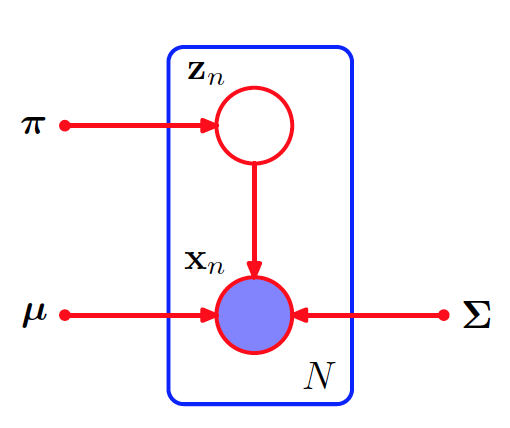
\includegraphics[width = 0.4\hsize]{./figures/GMM.png} 
		\caption{Gaussian Mixture Model.} % caption of the figure
		\label{fig:GMM} % a label. When we refer to this label from the text, the figure number is included automatically
	\end{center}
\end{figure}


\subsubsection{Formulation of the Gaussian Mixture Models}
Let $\vec{z}$ be a $K$-dimensional binary random variable with 1-of-$K$ representation.
\begin{align*}
	p(z_k=1) = \pi_k 	&\Rightarrow p(\vec{z})=\prod_{k=1}^K \pi_k^{z_k}
\end{align*}

Conditional probability of $\vec{x}$ given a particular value for latent variable $\vec{z}$:
\begin{align*}
	p(\vec{x}\vert \vec{z}) = \prod_{k=1}^K \mathcal{N}(\vec{x}\vert \vec{\mu}_k, \vec{\Sigma}_k)^{z_k}
\end{align*}

Using Bayes theorem and marginalize the latent variable $\vec{z}$
\begin{align*}
	p(\vec{x}) =\sum_{\vec{z}}p(\vec{z})p(\vec{x}\vert \vec{z}) = \sum_{k=1}^K \pi_k\mathcal{N}(\vec{x}\vert \vec{\mu}_k, \vec{\Sigma}_k)
\end{align*}

Similarly, the posterior probability of $\vec{z}$ is given by
\begin{align*}
	\gamma (z_k) = \frac{p(\vec{x}\vert z_k=1)p(z_k=1)}{p(\vec{x})} = \frac{\pi_k \mathcal{N}(\vec{x}\vert \vec{\mu}_k, \vec{\Sigma}_k) }{\sum_{j=1}^K \pi_j\mathcal{N}(\vec{x}\vert \vec{\mu}_j, \vec{\Sigma}_j)}
\end{align*}

\subsubsection{Maximum Likelihood}
The log-likelihood function is given by
\begin{align*}
	\ln p(\vec{X} \vert \vec{\pi}, \vec{\mu}, \vec{\Sigma})&=\sum_{n=1}^N \ln\left(\sum_{k=1}^K \pi_k\mathcal{N}(\vec{x}\vert \vec{\mu}_k, 	\vec{\Sigma}_k)\right)
\end{align*}

The maximum likelihood method will yield the following:
\begin{align*}
	\vec{\mu}_k & = \frac{\sum_{n=1}^N \gamma(z_{nk})\vec{x}_n}{\sum_{n=1}^N \gamma(z_{nk})}\\
	\vec{\Sigma}_k& = \frac{\sum_{n=1}^N \gamma(z_{nk})(\vec{x}_n-\vec{\mu}_k)(\vec{x}_n-\vec{\mu}_k)^\top}{\sum_{n=1}^N \gamma(z_{nk})}\\
	\pi_k&= \frac{\sum_{n=1}^N \gamma(z_{nk})}{N}
\end{align*}

Issues with maximum likelihood:
\begin{enumerate}
	\item Presence of singularities: When we have at least two components in the mixture, one of them can have a finite variance and assign finite probability to all the data points, while the other component can shrink onto one specific data point and therefore contribute to an ever increasing additive value to the log likelihood.
	\item Identifiability: Solutions may not be unique, hence it may be hard to interpret the parameter values discovered by a model.
	\item The log likelihood equation is difficult to optimize over.
\end{enumerate}


\subsubsection{Expectation Maximization Formulation}
Supposed that in addition to $\vec{X}$, we were also given the values of the latent variables $\vec{Z}$, the likelihood and the log likelihood function are given by
\begin{align*}
	p(\vec{X}, \vec{Z}\vert \vec{\mu}, \vec{\Sigma}, \vec{\pi})& =\prod_{n=1}^{N}\prod_{k=1}^{K} \pi_k^{z_{nk}}\mathcal{N}(\vec{x}_n\vert \vec{\mu}_k, \vec{\Sigma}_k)^{z_{nk}}\\
	\ln p(\vec{X}, \vec{Z}\vert \vec{\mu}, \vec{\Sigma}, \vec{\pi})& =\sum_{n=1}^{N}\sum_{k=1}^{K} z_{nk}\left(\ln \pi_k + \ln \mathcal{N}(\vec{x}_n\vert \vec{\mu}_k, \vec{\Sigma}_k)\right)
\end{align*}

\begin{enumerate}
\item \textbf{Expectation Step}:

Taking the expectation on the log likelihood 
\begin{align*}
\mathbb{E}_{p(\vec{Z}\vert \vec{X}, \vec{\theta})}\left[\ln p(\vec{X}, \vec{Z}\vert \vec{\mu}, \vec{\Sigma}, \vec{\pi})\right]
& =\sum_{n=1}^{N}\sum_{k=1}^{K} \mathbb{E}_{p(\vec{Z}\vert \vec{X}, \vec{\theta})}[z_{nk}]\left(\ln \pi_k + \ln \mathcal{N}(\vec{x}_n\vert \vec{\mu}_k, \vec{\Sigma}_k)\right)\\
& = G(\vec{\theta})
\end{align*}

\begin{align*}
p(\vec{Z}\vert \vec{X}, \vec{\theta})\propto &
\prod_{n=1}^N\prod_{k=1}^K [\pi_k\mathcal{N}(\vec{x}_n\vert \vec{\mu}_k, \vec{\Sigma}_k)]^{z_{nk}}
\end{align*}

\begin{align*}
\mathbb{E}_{p(\vec{Z}\vert \vec{X}, \vec{\theta})}[z_{nk}]
&= \frac{\sum_{z_{nk}}z_{nk}[\pi_k\mathcal{N}(\vec{x}_n\vert \vec{\mu}_k, \vec{\Sigma}_k)]^{z_{nk}} }{\sum_{j=1}^K \pi_j \mathcal{N}(\vec{x}_n \vert \vec{\mu}_j, \vec{\Sigma}_j)}\\
&= \frac{\pi_k \mathcal{N}(\vec{x}_n \vert \vec{\mu}_k, \vec{\Sigma}_k)}{\sum_{j=1}^K \pi_j \mathcal{N}(\vec{x}_n \vert \vec{\mu}_j, \vec{\Sigma}_j)}\\
&=\gamma({z_{nk}})
\end{align*}

\item \textbf{Maximization Step}:
By taking the derivative of $(\vec{\theta})$ w.r.t $\vec{\theta}$ and set them to $0$, the parameters can be found to be
\begin{align*}
	\vec{\mu}_k & = \frac{\sum_{n=1}^N \gamma(z_{nk})\vec{x}_n}{\sum_{n=1}^N \gamma(z_{nk})}\\
	\vec{\Sigma}_k& = \frac{\sum_{n=1}^N \gamma(z_{nk})(\vec{x}_n-\vec{\mu}_k)(\vec{x}_n-\vec{\mu}_k)^\top}{\sum_{n=1}^N \gamma(z_{nk})}\\
	\pi_k&= \frac{\sum_{n=1}^N \gamma(z_{nk})}{N}
\end{align*}

\end{enumerate}

\subsubsection{Expectation Maximization Algorithm}
Given a Gaussian mixture model, the goal is to maximize the likelihood functions w.r.t to the parameters:
\begin{enumerate}
	\item Initialize the means $\vec{\mu}_k$, covariances $\vec{\Sigma}_k$ and mixing coefficients $\pi_k$ and evaluate the initial of the log likelihood.
	\item E Step: Evaluate the responsibilities using the current parameter values
		\begin{align*}
			\gamma (z_k) = \frac{p(\vec{x}\vert \vec{z})p(\vec{z})}{p(\vec{x})} = \frac{\pi_k \mathcal{N}(\vec{x}\vert \vec{\mu}_k, \vec{\Sigma}_k) }	{\sum_{j=1}^K \pi_j\mathcal{N}(\vec{x}\vert \vec{\mu}_j, \vec{\Sigma}_j)}
		\end{align*}
	\item M Step: Re-estimate the parameters using the current responsibilities
		\begin{align*}
			\vec{\mu}_k^{new}&=\frac{1}{N_k}\sum_{n=1}^N \gamma(z_{nk})\vec{x}_n\\
			\vec{\Sigma}_k^{new}&=\frac{1}{N_k}\sum_{n=1}^N \gamma(z_{nk})(\vec{x}_n-\vec{\mu}_k)(\vec{x}_n-\vec{\mu}_k)^\top\\
			\pi_k^{new}&=\frac{N_k}{N}
		\end{align*}
	where
		\begin{align*}
			N_k & = \sum_{n=1}^N \gamma(z_{nk})
		\end{align*}
	\item Evaluate the log likelihood
		\begin{align*}
			\ln p(\vec{X} \vert \vec{\pi}, \vec{\mu}, \vec{\Sigma})&=\sum_{n=1}^N \ln\left(\sum_{k=1}^K \pi_k\mathcal{N}(\vec{x}\vert \vec{\mu}_k, 		\vec{\Sigma}_k)\right)
	\end{align*}
	and check for convergence of either parameter of the log likelihood. If the convergence criterion is not satisfied, return to step 2
\end{enumerate}


\subsection{Bernoulli Mixture Models}

\begin{align*}
p(\vec{x}\vert \vec{\mu}) & = \prod_{i=1}^D \mu_i^{x_i}(1-\mu_i)^{1-x_i}\\
\mathbb{E}[\vec{x}] & = \vec{\mu}\\
\mathbb{V}[\vec{x}] &= diag\lbrace \mu_i(1-\mu_i)\rbrace
\end{align*}

The mixture of the Bernoulli distributions is given by
\begin{align*}
p(\vec{x}\vert \vec{\mu}, \vec{\pi})&=\sum_{k=1}^K \pi_kp(\vec{x}\vert \vec{\mu}_k)\\
p(\vec{x}\vert \vec{\mu}_k) &= \prod^{D}_{i=1} \mu_{ki}^{x_i} (1- \mu_{ki}^{x_i})^{1-x_i}\\
\mathbb{E}[\vec{x}] & = \sum_{k=1}^K \pi_k\vec{\mu}_k\\
\mathbb{V}[\vec{x}] &= \sum_{k=1}^K \pi_k \left(\vec{\Sigma}_k + \vec{\mu}_k\vec{\mu}_k^\top\right) - \mathbb{E}[\vec{X}]\mathbb{E}[\vec{X}]^\top\\
\vec{\Sigma}_k & = diag\lbrace \mu_{ki}(1-\mu_{ki})\rbrace
\end{align*}

Let $\vec{z}$ be the one hot representation, we have
\begin{align*}
	p(\vec{x} \vert \vec{z}, \vec{\mu}) &= \prod_{k=1}^K p(\vec{x}\vert \vec{\mu}_k)^{z_k}\\
	p(\vec{z}\vert \vec{\pi}) &= \prod_{k=1}^K \pi_k^{z_k}
\end{align*}

The log likelihood function is given by
\begin{align*}
	\ln p(\vec{X}, \vec{Z} \vert \vec{\mu}, \vec{\pi})&=\sum_{n=1}^N\sum_{k=1}^Kz_{nk}
	\left\lbrace 
	\ln \pi_k +\sum_{i=1}^D[x_{ni}\ln\mu_{ki}+(1-x_{ni})\ln(1-\mu_{ki})]
	\right\rbrace
\end{align*}

The E step: we then take the expectation of the log likelihood above
\begin{align*}
\mathbb{E}_{\vec{Z}}[\ln p(\vec{X}, \vec{Z} \vert \vec{\mu}, \vec{\pi})]&=\sum_{n=1}^N\sum_{k=1}^K\gamma(z_{nk})
\left\lbrace 
\ln \pi_k +\sum_{i=1}^D[x_{ni}\ln\mu_{ki}+(1-x_{ni})\ln(1-\mu_{ki})]
\right\rbrace\\
&\\
\gamma(z_{nk})& = \frac{\sum_{z_{nk}} z_{nk}[\pi_kp(\vec{x}_n\vert \vec{\mu}_k)]^{z_{nk}} }{\sum_{z_{nj}}[\pi_jp(\vec{x}_n\vert \vec{\mu}_j)]^{z_{nj}}}
=\frac{\pi_kp(\vec{x}_n\vert \vec{\mu}_k)}{\sum_{j=1}^K \pi_jp(\vec{x)_n}\vert \vec{\mu}_j)}
\end{align*}

The M step: we then maximize the log likelihood wrt to the parameters
\begin{align*}
	\vec{\mu}_k &=\frac{1}{N_k}\sum_{n=1}^N \gamma(z_{nk})\\
	\pi_k&=\frac{N_k}{N}\\
	N_k &= \sum_{n=1}^N \gamma(z_{nk})
\end{align*}

\subsection{Convergence of the EM Algorithm}

\begin{align*}
	p(\vec{X} \vert \vec{\theta}) = \sum_{\vec{Z}} p(\vec{X},\vec{Z} \vert \vec{\theta}) &\Rightarrow \ln p(\vec{X} \vert \vec{\theta}) = \mathcal{L}(q, \vec{\theta}) + KL(q\parallel p)\\
	\mathcal{L}(q, \vec{\theta})&=\sum_{\vec{Z}} q(\vec{Z})\ln \left[\frac{p(\vec{X}, \vec{Z}\vert \vec{\theta})}{q(\vec{Z})}\right]\\
	 KL(q\parallel p)&=-\sum_{\vec{Z}} q(\vec{Z})\ln \left[\frac{p(\vec{Z}\vert \vec{X}, \vec{\theta})}{q(\vec{Z})}\right]
\end{align*}

In the E step, the lower bound $\mathcal{L}(q,\vec{\theta}^{old})$ is maximized with respect to $q(\vec{Z})$. The solution to this maximization problem can be done by setting $q(\vec{Z}) = p (\vec{Z}\vert \vec{X}, \vec{\theta}^{old})$ such that $KL(q\parallel p)=0$.\\

In the M step, the lower bound $\mathcal{L}(q,\vec{\theta}^{old})$ is maximized with respect to $\vec{\theta}$. However, the KL divergence will no longer be zero. Hence, the increase in the upper bound of the log likelihood function is greater than the increase in the lower bound.\\

By substituting $q(\vec{Z}) = p(\vec{Z}\vert\vec{X}, \vec{\theta}^{old})$, we get the lower bound to be the following after the E step:
\begin{align*}
	\mathcal{L}(q,\vec{\theta}) & = \sum_{\vec{Z}}p(\vec{Z}\vert \vec{X}, \vec{\theta}^{old})\ln p(\vec{X},\vec{Z}\vert \vec{\theta}) - \sum_{\vec{Z}}p(\vec{Z}\vert \vec{X}, 	\vec{\theta}^{old})\ln p(\vec{Z} \vert \vec{X}, \vec{\theta}^{old})\\
	&= \mathcal{Q}(\vec{\theta},\vec{\theta}^{old} ) + const 
\end{align*}


\newpage

\section{Probabilistic PCA}

\begin{align*}
	\vec{x} &= \vec{Wy} + \vec{\mu} + \vec{e}\\
	\vec{e} & \sim \mathcal{N}(\vec{e}\vert \vec{0}, \sigma^2\vec{I})\\
	\vec{y} & \sim \mathcal{N}(\vec{y}\vert \vec{0}, \vec{I})
\end{align*}


\begin{figure}[H]
\begin{center}
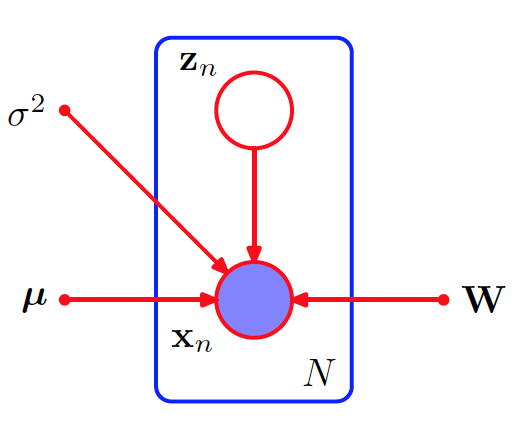
\includegraphics[width = 0.4\hsize]{./figures/PPCA.png} % this includes the figure and specifies that it should span 0.7 times the horizontal size of the 
\caption{Gaussian Mixture Model.} % caption of the figure
\label{fig:PPCA} % a label. When we refer to this label from the text, the figure number is included automatically
\end{center}
\end{figure}

\subsection{Maximum Likelihood}
\begin{enumerate}
\item We are interested in the distribution of $\vec{x}$ and the parameters $\vec{\theta}$. The marginal distribution of $\vec{x}$ can be obtained by integrating $\vec{y}$ out of the joint distribution.
\begin{align*}
p(\vec{x}_1,\dots, \vec{x}_N \vert \vec{\theta})
&=\int_{\vec{y_i}}p(\vec{x}_1,\dots, \vec{x}_N, \vec{y}_1,\dots, \vec{y}_N \vert \vec{\theta}) d\vec{y}_1\dots d\vec{y}_N\\
&= \int_{\vec{y_i}}\prod_{i=1}^N p(\vec{x}_i \vert \vec{y}_i,\vec{W}, \vec{\mu}, \sigma)p(\vec{y}_i)d\vec{y}_1\dots d\vec{y}_N\\
&= \prod_{i=1}^N\int_{\vec{y_i}} p(\vec{x}_i \vert \vec{y}_i,\vec{W}, \vec{\mu}, \sigma)p(\vec{y}_i)d\vec{y}_i
\end{align*}

\item The joint distribution can be obtained by applying Bayes' Rule.
\begin{align*}
p(\vec{x}_1,\dots, \vec{x}_N, \vec{y}_1,\dots, \vec{y}_N \vert \vec{\theta})
& = \prod_{i=1}^N p(\vec{x}_i \vert \vec{y}_i,\vec{W}, \vec{\mu}, \sigma)p(\vec{y}_i)\\
p(\vec{x}_i \vert \vec{y}_i,\vec{W}, \vec{\mu}, \sigma)p(\vec{y}_i) 
&= \left[(2\pi\sigma^2)^{-\frac{F}{2}} e^{-\frac{1}{2\sigma^2}(\vec{x}_i-\vec{\mu}-\vec{Wy}_i)^\top(\vec{x}_i-\vec{\mu}-\vec{Wy}_i)}\right]\left[(2\pi)^{-\frac{d}{2}}e^{-\frac{1}{2}\vec{y}_i^\top\vec{y}_i}\right]
\end{align*}

\item By collecting the $\vec{y}$ in the exponents, completing the squares and then applying the Woodbury identity (more details please refer to notes in 496):
\begin{align*}
p(\vec{x}_i\vert \vec{W}, \vec{\mu}, \sigma^2) & = \mathcal{N}(\vec{x}_i\vert \vec{\mu}, \vec{D} )\\
\vec{D}&=\vec{WW}^\top +\sigma^2\vec{I}\\
p(\vec{y}_i\vert \vec{x}_i, \vec{W}, \vec{\mu}, \sigma^2) & = \mathcal{N}(\vec{y}_i \vert \vec{M}^{-1}\vec{W}^\top(\vec{x}_i-\vec{\mu}), \sigma^2\vec{M}^{-1})\\
\vec{M}&=\sigma^2\vec{I} + \vec{W^\top W}
\end{align*}

\item  Maximizing the likelihood and solve for the parameters
\begin{align*}
\vec{S_t} & = \vec{U\Lambda U}^\top \text{ ($\vec{S_t}$ is the covariance matrix)}\\
\sigma^2 & = \frac{1}{F-d} \sum_{j= d+1}^F \lambda_j\\
\vec{W_d}&= \vec{U_d}(\vec{\Lambda} - \sigma^2\vec{I})^{\frac{1}{2}}\vec{V}^\top
\end{align*}

\item Hence we no longer have a projection but:
\begin{align*}
\mathbb{E}_{\vec{p(\vec{y}_i\vert \vec{x}_i)}} [\vec{y}_i] & = \vec{M}^{-1}\vec{W}^\top (\vec{x}_i - \vec{\mu})\\
\vec{\widehat{x}_i}&= \vec{W}\mathbb{E}_{\vec{p(\vec{y}_i\vert \vec{x}_i)}} [\vec{y}_i]  + \vec{\mu}
\end{align*}

\end{enumerate}


\subsection{EM PPCA}
\begin{enumerate}
\item Write the log likelihood of the joint distribution of the observed and latent variables
\begin{align*}
p(\vec{X,Y} \vert \vec{\theta}) &= \prod_{i=1}^N p(\vec{x}_i \vert\vec{y}_i, \vec{\theta})p(\vec{y}_i)\\
\ln p(\vec{X,Y} \vert \vec{\theta}) &= \sum_{i=1}^N \left(\ln p(\vec{x}_i \vert\vec{y}_i,\vec{\theta})+ \ln p(\vec{y}_i)\right)\\
\ln p(\vec{x}_i \vert \vec{y}_i, \vec{\theta}) &= -\frac{F}{2}\ln (2\pi\sigma^2) - \frac{1}{2\sigma^2}(\vec{x}_i-\vec{Wy}_i-\vec{\mu})^\top (\vec{x}_i-\vec{Wy}_i-\vec{\mu})\\
\ln p(\vec{y}_i)&= -\frac{1}{2}\vec{y}_i^\top \vec{y}_i-\frac{D}{2}\ln 2\pi
\end{align*}

\item \textbf{E-Step:} Take the expectation on the log likelihood on the joint distribution:
\begin{align*}
\ln p(\vec{X,Y} \vert \vec{\theta}) &=\sum_{i=1}^N\left[-\frac{F}{2}\ln 2\pi\sigma^2 -\frac{1}{2\sigma^2}(\vec{x}_i-\vec{Wy}_i-\vec{\mu})^\top (\vec{x}_i-\vec{Wy}_i-\vec{\mu}) -\frac{1}{2}\vec{y}_i^\top\vec{y}_i-\frac{D}{2}\ln 2\pi\right]
\end{align*}

Expanding the above and use the identities $\text{tr}\left[\vec{y}_i^\top \vec{WW}^\top \vec{y}_i\right]=\text{tr}\left[\vec{y}_i\vec{y}_i^\top \vec{WW}^\top \right]$
\begin{align*}
\mathbb{E}_{p(\vec{Y\vert X})} [\ln p(\vec{X,Y} \vert \vec{\theta})]
&=-\frac{NF}{2}\ln 2\pi\sigma^2 -\frac{ND}{2}\ln 2\pi\\
& -\sum_{i=1}^N\left\lbrace\frac{1}{2\sigma^2}\left[(\vec{x}_i-\vec{\mu})^\top (\vec{x}_i-\vec{\mu}) -2 (\vec{x}_i-\vec{\mu})^\top \vec{W} \mathbb{E}[\vec{y}_i] \right.\right.\\
&+\left.\left.\text{tr}\left[\mathbb{E}(\vec{y}_i\vec{y}_i^\top)\vec{W^\top W}\right]\right]+\frac{1}{2}\text{tr}\left[\mathbb{E}(\vec{y}_i^\top \vec{y}_i)\right]\right\rbrace
\end{align*}

We can obtain the moments of $\vec{y_i}$ from the earlier derivation of the PPCA
\begin{align*}
p(\vec{y}_i\vert \vec{x}_i, \vec{W}, \vec{\mu}, \sigma^2) & = \mathcal{N}(\vec{y}_i \vert \vec{M}^{-1}\vec{W}^\top(\vec{x}_i-\vec{\mu}), \sigma^2\vec{M}^{-1})\\
\vec{M}&=\sigma^2\vec{I} + \vec{W^\top W}\\
\mathbb{E}_{p(\vec{Y\vert X})}[\vec{y}_i]&=\vec{M}^{-1}\vec{W}^\top(\vec{x}_i-\vec{\mu})\\
\mathbb{E}_{p(\vec{Y\vert X})}[\vec{y}_i \vec{y}_i^\top]&=\sigma^2\vec{M}^{-1} +\mathbb{E}[\vec{y}_i]\mathbb{E}[\vec{y}_i]^\top
\end{align*}

\item \textbf{M-Step:} Maximize the log likelihood
\begin{align*}
\vec{\mu}&= \frac{1}{N}\sum_{i=1}^N(\vec{x}_i - \vec{W}\mathbb{E}[\vec{y}_i])\\
\vec{W}&=\left[\sum_{i=1}^N (\vec{x}_i - \vec{\mu})\mathbb{E}[\vec{y}_i]^\top]\right]\left[\sum_{i=1}^N \mathbb{E}[\vec{y}_i\vec{y}_i^\top]\right]^{-1}\\
\sigma^2&=\frac{1}{NF}\sum_{i=1}^N\left\lbrace \parallel \vec{x_i-\mu} \parallel^2 -2\mathbb{E}[\vec{y}_i]^\top\vec{W^\top (x_i-\mu)} +\text{tr}(\mathbb{E}[\vec{y}_i\vec{y}_i^\top]\vec{W^\top W})\right\rbrace
\end{align*}


\item Advantages of EM PPCA:
\begin{itemize}
\item A complexity of $O(NFD)$ can be significantly smaller than $O(NF^2)$ (from the computation of the covariance)
\item The EM procedure can be extended to factor analysis model
\item EM allows us to deal with missing values
\end{itemize}

\end{enumerate}


\section{PPCA Mixture Model}

\begin{figure}[H]
\begin{center}
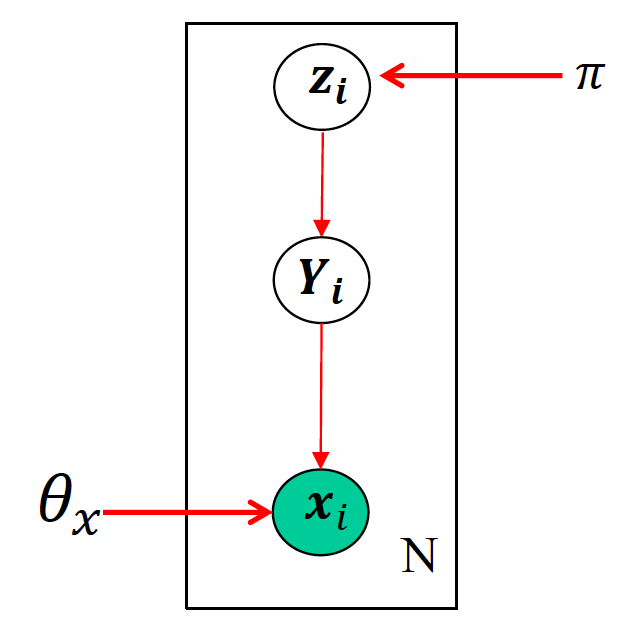
\includegraphics[width = 0.4\hsize]{./figures/PPCAMixture.png} % this includes the figure and specifies that it should span 0.7 times the horizontal size of the 
\caption{PPCA Mixture Model.} % caption of the figure
\label{fig:PPCA Mixture Model} % a label. When we refer to this label from the text, the figure number is included automatically
\end{center}
\end{figure}


The model is given by:
\begin{align*}
	\vec{x}_i &= \vec{\mu}_k + \vec{W}_k\vec{y}_{ik} + \vec{e}_{ik}\\
	\vec{y}_{ik} &\sim \mathcal{N} (\vec{y}_{ik}\vert \vec{0,I})\\
	\vec{e}_{ik} & \sim \mathcal{N} (\vec{e}_{ik}\vert \vec{0},\sigma^2_k\vec{I}), \forall k = 1,\dots, K\\
	p(\vec{x}_i\vert  \vec{z}_{ik} &=1, \vec{y}_{ik}, \vec{\mu_k}, \vec{W_k}, \sigma^2_k \vec{I}) = \mathcal{N}(\vec{x}_i \vert \vec{\mu}_k + \vec{W}_k\vec{y}_{ik})\\
	p(\vec{x}_i\vert \vec{\theta})& = \sum_{k=1}^K \pi_k \mathcal{N}(\vec{x}_i \vert \vec{\mu}_k, \vec{D}_k)\\\
	\vec{D}_k &= \vec{W}_k\vec{W}_k^\top + \sigma_k^2\vec{I}
\end{align*}


\subsection{Probability Distributions for EM Formulation}

\begin{enumerate}
\item Priors distributions:
	\begin{align*}
		p(\vec{z}_i \vert \vec{\theta}_z) & = \prod_{k=1}^K \pi_k^{z_{ik}}\\
		p(\vec{Y}_i \vert \vec{z}_i, \vec{\theta}_z) & = \prod_{k=1}^K p(y_{ik})^{z_{ik}} = \prod_{k=1}^K \mathcal{N}(y_{ik}\vert \vec{0}, \vec{I})^{z_{ik}}
	\end{align*}

\item Conditional distribution:
	\begin{align*}
		p(\vec{x}_i \vert \vec{z}_i, \vec{Y}_i, \vec{\theta_x}) 
		& = \prod_{k=1}^K p(\vec{x}_i \vert \vec{z}_{ik}=1, \vec{y}_{ik}, \vec{W}_k, \vec{\mu}_k, \vec{\sigma}_k^2\vec{I})^{z_{ik}}\\
		& = \prod_{k=1}^K \mathcal{N}(\vec{x}_{ik}\vert \vec{W}_k \vec{y}_{ik}+\vec{\mu}_k, \sigma_k\vec{I})^{z_{ik}}		
	\end{align*}

\item Marginal distributions per cluster is found by integrating $\vec{y}$ out:
	\begin{align*}
		p(\vec{x}_i \vert \vec{z}_{ik}=1, \vec{W}_k, \vec{\mu}_k, \sigma_k^2) = \mathcal{N}(\vec{x}_i\vert \vec{\mu}_k, \vec{D}_k)\\
		\vec{D}_k = \vec{W}_k\vec{W}_k^\top + \sigma_k^2 \vec{I}
	\end{align*}

\item Full marginal distributions:
	\begin{align*}
		p(\vec{x}_i \vert \vec{\theta}) 
		&= \sum_{k=1}^K p(z_{ik}=1)p(\vec{x}\vert z_{ik}=1, \theta_x)\\
		&= \sum_{k=1}^K \pi_k \mathcal{N}(\vec{x}_i\vert \vec{\mu}_k, \vec{D}_k)		
	\end{align*}

\item Posteriors on $\vec{y}_{ik}$ (we will take expectation on this in the E step):
	\begin{align*}
		p(\vec{y}_{ik} \vert \vec{x}_{ik}, z_{ik}=1, \vec{W}_{k}, \vec{\mu}_{k}, \sigma_k^2 )
		&= \mathcal{N}\left(\vec{y}_{ik}\vert \vec{M}_k^{-1}\vec{W}_k^\top(\vec{x}_i - \vec{\mu}_k),\sigma_k^2 \vec{M}_k^{-1}\right)\\
		\mathbb{E}(\vec{y}_{ik})& = \vec{M}_k^{-1}\vec{W}_k^\top (\vec{x}_i - \vec{\mu}_k)\\
		\mathbb{E}(\vec{y}_{ik}\vec{y}_{ik}^\top)& =\sigma_k^2\vec{M}_k^{-1}+\mathbb{E}(\vec{y}_{ik})\mathbb{E}(\vec{y}_{ik})^\top
	\end{align*}

\item Posteriors on $\vec{z}_i$  (we will take expectation on this in the E step):
\begin{align*}
p(\vec{z}_i \vert \vec{x}_i, \theta)
&= \frac{p(\vec{x}_i, \vec{z}_i \vert \theta)}{p(\vec{x}_i \vert \theta)}
= \frac{p(\vec{x}_i\vert \vec{z}_i, \theta)p(\vec{z}_i \vert \theta)}{p(\vec{x}_i \vert \theta)}
= \frac{\prod_k^K \left(\mathcal{N}(\vec{x}_i \vert \vec{\mu}_k, \vec{D}_k)\pi_k\right)^{z_{nk}}}{\sum_{l =1}^K \pi_l \mathcal{N}(\vec{x}_i \vert \vec{D}_l, \vec{\mu}_l)}\\
\mathbb{E}[z_{ik}] & = \sum_{z_{ik}=0,1} z_{ik} p(\vec{z_i}\vert \vec{x}_i, \theta)
= \frac{\pi_k\mathcal{N}(\vec{x}_i \vert \vec{\mu}_k, \vec{D}_k)}{\sum_{l=1}^K \pi_l\mathcal{N}(\vec{x}_i \vert \vec{\mu}_l, \vec{D}_l)}
\end{align*}

\end{enumerate}


\subsection{Formulation of EM}
\begin{enumerate}
\item Setting the joint likelihood (decomposition below can be guided by graphical model):	
	\begin{align*}
	p(\vec{X}, \vec{Y}, \vec{Z} \vert \theta) 
	&= p(\vec{X} \vert \vec{Z}, \vec{Y}, \theta_x)p(\vec{Z}, \vec{Y}\vert \theta_Z)
	= p(\vec{X} \vert \vec{Z}, \vec{Y}, \theta_x)p(\vec{Y}\vert \vec{Z})p(\vec{Z}\vert \theta_Z)\\
	p(\vec{Z}\vert \theta_Z)
	&= \prod_{i=1}^N \prod_{k=1}^K \pi_k^{z_{ik}}\\
	p(\vec{Y}\vert \vec{Z})
	&= \prod_{i=1}^N p(\vec{Y}_i\vert \vec{z}_i, \theta_Z)
	= \prod_{i=1}^N \prod_{k=1}^3 p(\vec{y}_{ik})^{z_{ik}}
	= \prod_{i=1}^N \prod_{k=1}^3 \mathcal{N}(\vec{y}_{ik}\vert \vec{0}, \vec{I})^{z_{ik}}\\
	p(\vec{X} \vert \vec{Z}, \vec{Y}, \theta_x)
	&=\prod_{i=1}^N p(\vec{x}_i \vec{z}_i, \vec{Y}_i, \theta_x
	=\prod_{i=1}^N\prod_{k=1}^K \mathcal{N}(\vec{x}_i \vert \vec{W}_k\vec{y}_{ik}+\vec{\mu}_k, \sigma_k^2)^{z_{ik}}
	\end{align*}
	
	
	
Hence the log likelihood of the joint distribution:
\begin{align*}
\ln p(\vec{X}, \vec{Z}, \vec{Y} \vert \theta) 
&=\sum_{i=1}^N \sum_{k}^K z_{ik}\left[\ln  \mathcal{N}(\vec{x}_i \vert \vec{W}_k\vec{y}_{ik}+\vec{\mu}_k, \sigma_k^2) + \ln \mathcal{N}(\vec{y}_{ik}\vert \vec{0}, \vec{I}) + \ln\pi_k\right]\\
&= \sum_{i=1}^N \sum_{k}^K z_{ik}\left[-\frac{1}{2\sigma_k^2}(\vec{x}_i - \vec{\mu}_k - \vec{W}_k\vec{y}_k)^\top(\vec{x}_i - \vec{\mu}_k - \vec{W}_k\vec{y}_k)-\frac{F}{2}\ln 2\pi - F\ln\sigma_k\right]\\
&+ \sum_{i=1}^N\sum_{k}^K z_{ik}\left[-\frac{1}{2}\vec{y}_{ik}^\top\vec{y}_{ik} - \frac{d}{2}\ln 2\pi\right]+\sum_{i=1}^N\sum_{k}^K z_{ik}\ln \pi_k
\end{align*}

\item Taking the expectation yields
\begin{align*}
&\mathbb{E}[\ln p(\vec{X}, \vec{Z}, \vec{Y} \vert \theta) ]\\
&=-\frac{1}{2\sigma_k^2} \sum_{i=1}^N \sum_{k}^K \mathbb{E}[z_{ik}]\left[
\parallel \vec{x}_i -\vec{\mu}_k\parallel^2 - \mathbb{E}[\vec{y}_{ik}]^\top\vec{W}_k^\top(\vec{x}_i-\vec{\mu}_k) + \text{tr}(\vec{WW}^\top \mathbb{E}[\vec{y}_{ik}\vec{y}_{ik}^\top])\right]\\
&+\sum_{i=1}^N\sum_{k}^K\left[\frac{F}{2}\ln 2\pi - F\ln\sigma_k\right]+ \sum_{i=1}^N\sum_{k}^K \mathbb{E}[z_{ik}]\left[-\frac{1}{2}\text{tr}(\mathbb{E}[\vec{y}_{ik}\vec{y}_{ik}^\top]) - \frac{d}{2}\ln 2\pi\right]+\sum_{i=1}^N\sum_{k}^K \mathbb{E}[z_{ik}]\ln \pi_k
\end{align*}

\item The maximization step:
\begin{align*}
\pi_k &= \frac{1}{N}\sum^N_{i=1} \mathbb{E}[z_{ik}]\\
\vec{\mu}_k &= \frac{\sum_{i=1}^N \mathbb{E}[z_{ik}](\vec{x}_i - \vec{W}_k \mathbb{E}[\vec{y}_{ik}])} {\sum_{i=1}^N \mathbb{E}[z_{ik}]}\\
\vec{W}_k & = \left[\sum_{i=1}^N\mathbb{E}[z_{ik}](\vec{x}_i - \vec{\mu})\mathbb{E}[\vec{y}_{ik}^\top]\right]\left[\sum_{i=1}^N\mathbb{E}[z_{ik}]\mathbb{E}[\vec{y_{ik}}\vec{y}_{ik}^\top])  \right]^{-1}\\
\sigma_k^2 = \frac{1}{F\sum_{i=1}^N \mathbb{E}[z_{ik}]}&\sum_{i=1}^N \mathbb{E}[z_{ik}]\left[\parallel\vec{x}_i-\vec{\mu}_k\parallel^2 - \mathbb{E}[\vec{y}_{ik}]^\top \vec{W}^\top_k(\vec{x}_i-\vec{\mu}_k) + \text{tr}\left(\vec{W}_k^\top \vec{W}_k \mathbb{E}[\vec{y}_{ik}\vec{y}_{ik}^\top]\right)\right]
\end{align*}

\end{enumerate}

\newpage

\section{PPCA with Missing Values}
Given the PPCA model:
\begin{align*}
\vec{x} &= \vec{Wy} + \vec{\mu} + \vec{e}\\
\vec{e} & \sim \mathcal{N}(\vec{e}\vert \vec{0}, \sigma^2\vec{I})\\
\vec{y} & \sim \mathcal{N}(\vec{y}\vert \vec{0}, \vec{I})
\end{align*}
\begin{align*}
p(\vec{x}_i \vert \vec{W}, \vec{\mu}, \sigma^2)&= \mathcal{N}(\vec{x}_i\vert \vec{\mu}, \vec{D})\\
p(\vec{y}_i \vert \vec{x}_i, \vec{W}, \vec{\mu}, \sigma^2)&=\mathcal{N}(\vec{y}_i \vert \vec{M}^{-1}\vec{W}^\top (\vec{x}_i-\vec{\mu}), \sigma^2\vec{M}^{-1})\\
\vec{D} &= \vec{WW}^\top +\sigma^2\vec{I} \\
\vec{M} &= \vec{W}^\top \vec{W} +\sigma^2\vec{I}
\end{align*}

\begin{enumerate}

	\item We can reformulate the PPCA model to take into account of missing data:
		\begin{align*}
			\vec{x} = 	\begin{bmatrix}
								\vec{x}^o \\ \vec{x}^u
							\end{bmatrix}
			&\Rightarrow
			p\left(\vec{x}^o, \vec{x}^u\right) = \mathcal{N}\left(\left.
				\begin{bmatrix}
					\vec{x}^o \\ \vec{x}^u
				\end{bmatrix}
			\right\vert 
				\begin{bmatrix}
					\vec{\mu}^o \\ \vec{\mu}^u
				\end{bmatrix},
				\begin{bmatrix}
					\vec{D}^{oo} 		&\vec{D}^{ou} 		\\ 
					\vec{D}^{uo}			&\vec{D}^{uu}
				\end{bmatrix}\right)\\
				p(\vec{x}^u\vert \vec{x}^o)
				&=\mathcal{N}\left(\vec{x}^u\left \vert\vec{\mu}^u +\vec{D}_{uo}\vec{D}_{oo}^{-1}(\vec{x}^o - \vec{\mu}^o), \vec{D}_{uu}-\vec{D}_{uo}\vec{D}_{oo}^{-1}\vec{D}_{ou}  				\right.\right )
\end{align*}

	\item For convenience, we can rewrite this formulation as derive its first order and second order moments:
		\begin{align*}
			p(\vec{x}_i\vert \vec{x}_i^o)  &= \mathcal{N} \left(\vec{x}_i\left\vert \vec{z}_i, \vec{Q}\right. \right)\\
			\vec{z}_i &=\begin{bmatrix}
			\vec{x}_i^o\\
			\vec{\mu}^u +\vec{D}_{uo}\vec{D}_{oo}^{-1}(\vec{x}^o - \vec{\mu}^o)
			\end{bmatrix}\\
			\vec{Q} & = \begin{bmatrix}
			0	&	0\\
			0	& 	\vec{D}_{uu}-\vec{D}_{uo}\vec{D}_{oo}^{-1}\vec{D}_{ou} 
			\end{bmatrix}
		\end{align*}		
		
		\begin{align*}
			\mathbb{E}_{p(\vec{x}_i\vert \vec{x}_i^o)}[\vec{x}_i] &=\vec{z}_i\\
			\mathbb{E}_{p(\vec{x}_i\vert \vec{x}_i^o)}[\vec{x}_i\vec{x}_i^\top] &=\vec{Q}+\vec{z}_i\vec{z}_i^\top\\
			\mathbb{E}_{p(\vec{x}_i\vert \vec{x}_i^o)}[(\vec{x}_i-\vec{a})(\vec{x}_i-\vec{a})^\top] &=\vec{Q}+(\vec{z}_i-\vec{a})(\vec{z}_i-\vec{a})^\top\\ 
		\end{align*}
		
	\item Writing down the log likelihood for the observed variable $X$ and the latent variable $Y$
		\begin{align*}
			\ln p(\vec{X}, \vec{Y} \vert \vec{\theta})
			&= -\frac{1}{2\sigma^2}\sum_{i=1}^N \left\lbrace\text{tr}\left[(\vec{x}_i-\vec{\mu})(\vec{x}_i-\vec{\mu})^\top\right]-  2\text{tr} \left[\vec{y}_i(\vec{x}_i-\vec{\mu})^\top \vec{W}\right]+\text{tr}\left[\vec{W}^\top\vec{Wy}_i\vec{y}_i^\top\right]\right\rbrace\\
			&-\frac{1}{2}\sum_{i=1}^N \text{tr}[\vec{y}_i\vec{y}_i^\top]-\frac{NF}{2} \ln 2\pi - NF \ln \sigma - N \ln 2\pi
		\end{align*}
	
	\item Take the expectation with regards to the probability distribution $p(\vec{X}, \vec{Y} \vert \vec{X}^o)$
		\begin{align*}
			&\mathbb{E}_{p(\vec{x}_i,\vec{y}_i\vert \vec{x}_i^o)}\left[\ln p(\vec{X}, \vec{Y} \vert \vec{\theta})\right]\\
			&= -\frac{1}{2\sigma^2}\sum_{i=1}^N \left\lbrace\text{tr}\left(\mathbb{E}\left[(\vec{x}_i-\vec{\mu})(\vec{x}_i-\vec{\mu})^\top\right]\right)-  2\text{tr} \left(\mathbb{E}\left[\vec{y}_i(\vec{x}_i-\vec{\mu})^\top\right] \vec{W}\right)+\text{tr}\left(\vec{W}^\top\vec{W}\mathbb{E}\left[\vec{y}_i\vec{y}_i^\top\right]\right)\right\rbrace\\
			&-\frac{1}{2}\sum_{i=1}^N \text{tr}\left(\mathbb{E}\left[\vec{y}_i\vec{y}_i^\top\right]\right)-\frac{NF}{2} \ln 2\pi - NF \ln \sigma - N \ln 2\pi
		\end{align*}
		
		\begin{align*}
			\mathbb{E}_{p(\vec{x}_i,\vec{y}_i\vert \vec{x}_i^o)}[(\vec{x}_i-\vec{\mu})(\vec{x}_i-\vec{\mu})^\top] 
			&=\mathbb{E}_{p(\vec{x}_i,\vec{y}_i\vert \vec{x}_i^o)}[(\vec{x}_i-\vec{\mu})(\vec{x}_i-\vec{\mu})^\top]\\ 
			&=\vec{Q}+(\vec{z}_i-\vec{\mu})(\vec{z}_i-\vec{\mu})^\top\\ 			
			\mathbb{E}_{p(\vec{x}_i,\vec{y}_i\vert \vec{x}_i^o)}[\vec{y}_i(\vec{x}_i-\vec{\mu})^\top] 
			&=\mathbb{E}_{p(\vec{x}_i\vert \vec{x}_i^o)}\left[\mathbb{E}_{p(\vec{y}_i\vert \vec{x}_i^o)} \left[\vec{y}_i(\vec{x}_i-\vec{\mu})^\top\right]\right] \\
			&=\mathbb{E}_{p(\vec{x}_i\vert \vec{x}_i^o)}\left[\vec{M}^{-1}\vec{W}^\top (\vec{x}_i-\vec{\mu})(\vec{x}_i-\vec{\mu})^\top\right]\\
			& =\vec{M}^{-1}\vec{W}^\top \mathbb{E}_{p(\vec{x}_i\vert \vec{x}_i^o)}\left[(\vec{x}_i-\vec{\mu})(\vec{x}_i-\vec{\mu})^\top\right]\\
			\mathbb{E}_{p(\vec{x}_i,\vec{y}_i\vert \vec{x}_i^o)}[\vec{y}_i\vec{y}_i^\top] 
			&=\mathbb{E}_{p(\vec{x}_i\vert \vec{x}_i^o)}\left[\mathbb{E}_{p(\vec{y}_i\vert \vec{x}_i^o)} \left[\vec{y}_i\vec{y}_i^\top\right]\right] \\
			&=\mathbb{E}_{p(\vec{x}_i\vert \vec{x}_i^o)}\left[\sigma^2 \vec{M}^{-1}+\vec{M}^{-1}\vec{W}^\top (\vec{x}_i-\vec{\mu})(\vec{x}_i-\vec{\mu})^\top\vec{W}\vec{M}^{-1}\right]\\
			& =\sigma^2\vec{M}^{-1}+ \vec{M}^{-1}\vec{W}^\top\mathbb{E}_{p(\vec{x}_i\vert \vec{x}_i^o)}\left[(\vec{x}_i-\vec{\mu})(\vec{x}_i-\vec{\mu})^\top\right] \vec{W} \vec{M}^{-1}
		\end{align*}

	\item Maximization step:
		\begin{align*}
				\vec{\mu}	&=\frac{1}{N}\sum_{i=1}^N \vec{z}_i\\
				\vec{W}	&=\left[\sum_{i=1}^N\mathbb{E}\left[(\vec{x}_i-\vec{\mu})\vec{y}_i^\top\right]\right]\left[\sum_{i=1}^N\mathbb{E}\left[\vec{y}_i\vec{y}_i^\top\right]\right]^{-1}\\
				\sigma^2 &=\frac{1}{NF}\sum_{i=1}^N\left\lbrace \text{tr}\left(\mathbb{E}\left[(\vec{x}_i-\vec{\mu})(\vec{x}_i-\vec{\mu})^\top\right]\right) 
				-2 \text{tr}\left( \mathbb{E} \left[ \vec{y}_i (\vec{x}_i-\vec{\mu})^\top \right]\vec{W} \right)
				+ \text{tr}\left(\mathbb{E}\left[\vec{y}_i\vec{y}_i^\top\right]\vec{W}^\top\vec{W}\right)	
				\right\rbrace\\
				\vec{D} & = \vec{W}\vec{W}^\top +\sigma^2\vec{I}
		\end{align*}			
	

\end{enumerate}

\newpage


\section {Hidden Markov Model}
\subsection{Preliminary: Markov Chains}

\begin{enumerate}
	\item Markov Property:
		\begin{align*}
			p(\vec{x_i} \vert \vec{x}_1, \ldots, \vec{x}_{i-1}) &= p(\vec{x}_i \vert \vec{x}_{i-1})
		\end{align*}
		
	\item Markov Model: Given the observations $\lbrace \vec{x}_t \rbrace_{t=1}^N$
		\begin{align*}
			p(\vec{x}_1, \ldots, \vec{x}_N) &= p(\vec{x}_1)\prod_{t=2}^N p(\vec{x}_t \vert \vec{x}_{t-1}) & \text{bigram model}\\
			p(\vec{x}_1, \ldots, \vec{x}_N) &= p(\vec{x}_1)p(\vec{x}_2\vert \vec{x}_1 )\prod_{t=3}^N p(\vec{x}_t \vert \vec{x}_{t-1},\vec{x}_{t-2}) & \text{trigram model}\\
			p(\vec{x}_1, \ldots, \vec{x}_N) &= p(\vec{x}_1)p(\vec{x}_2\vert \vec{x}_1 )p(\vec{x}_3\vert \vec{x}_1,\vec{x}_2 )\prod_{t=4}^N p(\vec{x}_t \vert \vec{x}_{t-1},\vec{x}_{t-2},\vec{x}_{t-3}) & \text{n-gram model}
		\end{align*}	
		
		\item A transition matrix $\vec{A}$ specifies the probabilities of getting from state $i$ (\textit{row}) to state $j$ (\textit{column}) in one step. Note that $\vec{A}$ is a stochastic matrix, i.e. the row must sum to 1.
		
		\item Stationary distribution is the long term distribution over the states
					\begin{align*}
						\vec{\pi}^\top & = \vec{\pi}^\top  \vec{A}\\
					\end{align*}
				Solving for the stationary distribution is the same as eigenanalysis, where $\vec{\pi}$ is an eigenvector with eigenvalue 1.	
				
				\begin{align*}
					\vec{\pi}^\top(\vec{I} - \vec{A}) = \vec{0}\\
					\vec{\pi}^\top \vec{1} = \vec{1}	
				\end{align*}
				
		\item For a stationary distribution to exist, the markov chain has to be irreducible and aperiodic.
			\begin{itemize}
				\item Irreducibility: The state transition diagram must be singly connected, i.e. it is possible to move from one state to another ($a_{ij}(t)>0$)
				\item Aperiodicity: $d(i) = gcd\lbrace t: a_{ii}(t)>0\rbrace =1, \forall i$. At some point in time, the probability of a recurrent connection is greater than 0.
			\end{itemize}
	
		\item \textbf{Detailed balance condition}: A markov process is called a reversible Markov process if it satisfies the detailed balance equations.
			\begin{align*}
				\pi_i P_{ij} = \pi_j P_{ji}
			\end{align*}
	
		\item Estimation of the transition matrix from training data (language model)\\
			\begin{enumerate}
				\item The probability of a character is given by
					\begin{align*}
						p(\vec{x}_1\vert \vec{\pi}) & = \prod_{k=1}^K \pi_k^{x_{1k}}\\
						p(\vec{x}_t\vert \vec{x}_{t-1}) & = \prod_{j=1}^K \prod_{k=1}^K a_{jk}^{x_{(t-1)j}x_{tk}}				
					\end{align*}
					
				\item Probability of a sequence $D_l$ with length $T$
					\begin{align*}
						P(D_l\vert \theta) 
						 = p(\vec{x}_1^l, \ldots, \vec{x}_T^l)
						 = p(\vec{x}_1^l) \prod_{t=2}^T p(\vec{x}_t^l \vert \vec{x}_{t-1}^l)
						 = \prod_{k=1}^K \pi_k^{x_{1k}^l}\prod_{t=2}^T\prod_{j=1}^K \prod_{k=1}^K a_{jk}^{x^l_{(t-1)j}x^l_{tk}}	
					\end{align*}
					
				\item The likelihood function is then
					\begin{align*}
						p(D_1,\ldots, D_N\vert \theta) 
						& = \prod_{l=1}^N p(D_l\vert \theta)
						 = \prod_{l=1}^N \left\lbrace  \prod_{k=1}^K \pi_k^{x_{1k}^l}\prod_{t=2}^T\prod_{j=1}^K \prod_{k=1}^K a_{jk}^{x^l_{(t-1)j}x^l_{tk}} \right\rbrace
					\end{align*}
					
					\begin{align*}
						\ln p(D_1,\ldots, D_N\vert \theta) 
						& =\sum_{l=1}^N\sum_{k=1}^K x_{1k}^l\ln\pi_k +\sum_{l=1}^N\sum_{t=2}^T\sum_{j=1}^K \sum_{k=1}^K x^l_{(t-1)j}x^l_{tk}\ln a_{jk}\\
						& = \sum_{k=1}^K \left(\sum_{l=1}^N x_{1k}^l\right)\ln\pi_k +\sum_{j=1}^K \sum_{k=1}^K\left(\sum_{l=1}^N\sum_{t=2}^T x^l_{(t-1)j}x^l_{tk}\right)\ln a_{jk}\\
						& = \sum_{k=1}^K N_k^1 \ln \pi_k + \sum_{j=1}^K \sum_{k=1}^K N_{jk} \ln a_{jk}
					\end{align*}
					
					where 
					\begin{align*}
						N_k^1& = \sum_{l=1}^N x_{1k}^l & N_{jk}&=\sum_{l=1}^N\sum_{t=2}^T x^l_{(t-1)j}x^l_{tk}
					\end{align*}

				\item We just need to solve the optimization below by formulating the Lagrangian:
					\begin{align*}
						\max_{\vec{\theta}}	&\sum_{k=1}^K N_k^1 \ln \pi_k + \sum_{j=1}^K \sum_{k=1}^K N_{jk} \ln a_{jk}\\
						\text{s.t. }&	\sum_{k=1}^K \pi_k =1\\
										&	\sum_{k=1}^K a_{jk} = 1
					\end{align*}									
					
					\begin{align*}
						\pi_k &= \frac{N_k^1}{\sum_{k=1}^K N_k^1}	&	a_{jk} & =\frac{N_{jk}}{\sum_{k=1}^K N_{jk}}
					\end{align*}
				
			\end{enumerate}					
				
\end{enumerate}


\subsection{Hidden Markov Model}

\subsubsection{Model Description and Important Properties}
\begin{figure}[H]
	\begin{center}
		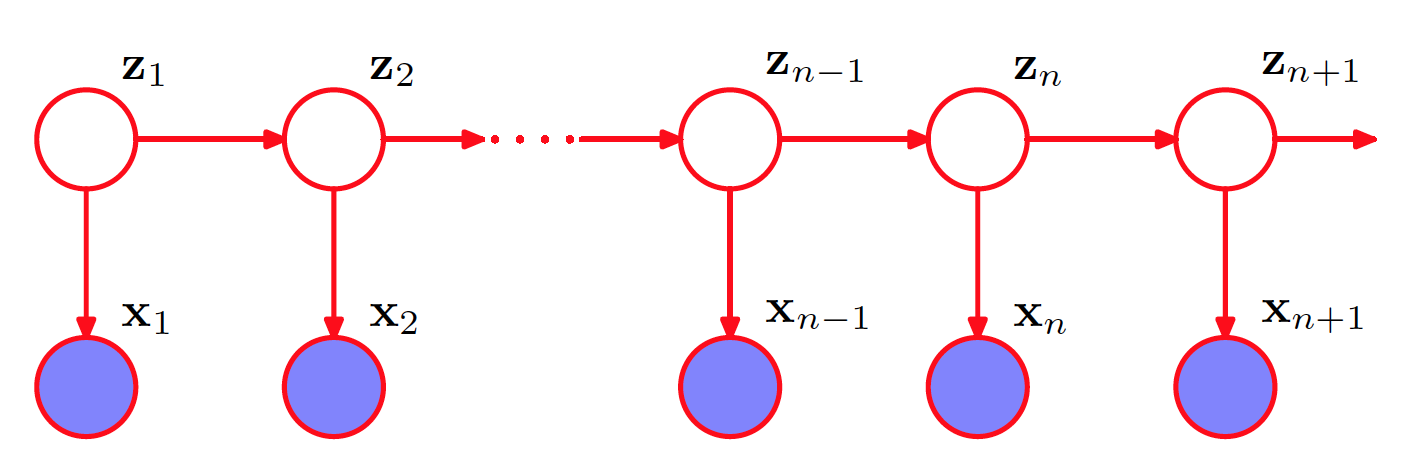
\includegraphics[width = 0.7\hsize]{./figures/HiddenMarkovModel.png} % this includes the figure and specifies that it should span 0.7 times the horizontal size of the 
		\caption{State Space Model. If $\vec{z}$ are discrete and markovian, then it is a Hidden Markov model.} % caption of the figure
		\label{fig:Hidden Markov Model} % a label. When we refer to this label from the text, the figure number is included automatically
	\end{center}
\end{figure}


\begin{enumerate}
	\item The HMM is a specific instance of the state space model in Figure \ref{fig:Hidden Markov Model} in which the latent variables are discrete.
	\item If we view a single time slice of the model, it corresponds to a mixture distribution densities given by $p(\vec{x}\vert \vec{z})$, where $p(\vec{z}_n \vert \vec{z}_{n-1})$.
	\item Properties of conditional independence
	\begin{align*}
		p(\vec{X}\vert \vec{z}_n)	 &= p(\vec{x}_1,\ldots, \vec{x}_n\vert \vec{z}_n)p(\vec{x}_{n+1},\ldots, \vec{x}_N\vert \vec{z}_n)\\
		p(\vec{x}_1,\ldots, \vec{x}_{n-1} \vert \vec{x}_n, \vec{z}_n)	&= p(\vec{x}_1,\ldots, \vec{x}_{n-1}\vert \vec{z}_n)\\
		p(\vec{x}_1,\ldots, \vec{x}_{n-1} \vert \vec{z}_{n-1}, \vec{z}_n)	&= p(\vec{x}_1,\ldots, \vec{x}_{n-1}\vert \vec{z}_{n-1})\\
		p(\vec{x}_{n+1},\ldots, \vec{x}_N \vert \vec{z}_n, \vec{z}_{n+1})&= p(\vec{x}_{n+1},\ldots, \vec{x}_N \vert \vec{z}_{n+1})\\
		p(\vec{x}_{n+2},\ldots, \vec{x}_N \vert \vec{z}_{n+1}, \vec{x}_{n+1})	& =p(\vec{x}_{n+2},\ldots, \vec{x}_N \vert \vec{z}_{n+1})\\
		p(\vec{X}\vert \vec{z}_{n-1}, \vec{z}_n) & = p(\vec{x}_1,\ldots, \vec{x}_{n-1}\vert \vec{z}_{n-1})p(\vec{x}_n\vert\vec{z}_n)p(\vec{x}_{n+1},\ldots, \vec{x}_N\vert \vec{z}_n)\\
		p(\vec{x}_{N+1}\vert \vec{X}, \vec{z}_{N+1})& = p(\vec{x}_{N+1}\vert \vec{z}_{N+1})\\
		p(\vec{z}_{N+1}\vert \vec{z}_N, \vec{X})	& = p(\vec{z}_{N+1}\vert \vec{z}_N)
	\end{align*}		
	
	\item Inferences using the Hidden Markov Model
		\begin{itemize}
			\item \textbf{Filtering}: Compute the belief state $p(\vec{z}_n \vert \vec{x}_1,\ldots, \vec{x}_n)$ online as the data streams in. It is known as filtering to reduce the noise in the estimation of the hidden state.
			
			\item \textbf{Smoothing}: Compute $p(\vec{z}_t\vert  \vec{x}_1,\ldots, \vec{x}_N)$ offline, given all the evidence. Reducing the uncertainty by conditioning on the past and future data. 
			
			\item \textbf{Fixed lag smoothing}: Compute  $p(\vec{z}_{t-\ell} \vert \vec{x}_1,\ldots, \vec{x}_n)$, where  $\ell >0$ is the lag. 
			
			\item \textbf{MAP estimation}: Compute $\text{arg} \max_{\vec{z}_1,\ldots, \vec{z}_n} p(\vec{z}_{1},\ldots,\vec{z}_{n} \vert \vec{x_1}, \ldots, \vec{x_n}) $. This is known as Viterbi Decoding.
			
			\item \textbf{Evaluation}: Find the probability of the evidence $p(\vec{x}_1,\ldots, \vec{x}_N)= \sum_{\vec{z}} p(\vec{x}, \vec{z})$.			
			
			\item \textbf{Prediction}: Predicting the future given the past, we compute $p(\vec{z}_{n+\delta}\vert \vec{x}_1, \ldots, \vec{x}_n)$ and $p(\vec{x}_{n+\delta}\vert \vec{x}_1, \ldots, \vec{x}_n)$.
			
			\item \textbf{Parameter Estimation}: This is know as the Baum-Welch algoritm. We estimate the parameter $\vec{A}$, $\vec{\pi}$ and $\vec{\theta}$.
		\end{itemize}

\end{enumerate}


\subsubsection{Formulation (Discrete Case)}
Let there be $K$ possible states for the latent variable $\vec{z}$ and $S$ possible states for the observed variable $\vec{x}$.
\begin{align*}
	p(\vec{z}_1\vert \vec{\pi}) 						&= \prod_{c=1}^K \pi_c^{z_{1,c}}\\
	p(\vec{z}_n \vert \vec{z}_{n-1}, \vec{A})	&= \prod_{i=1}^K \prod_{j=1}^K a_{ij}^{z_{n-1, i}z_{n, j}}\\
	p(\vec{x}_n \vert \vec{z}_n)					 	&= \prod_{i=1}^S \prod_{j=1}^K b_{ij}^{x_{n,i}z_{n,j}}
\end{align*}

If $\vec{x}$ is continuous, we just replace the last equation as
\begin{align*}
	p(\vec{x}_n \vert \vec{z}_n)	 = \prod_{j=1}^K p(\vec{x}_n \vert \vec{z}_{n, j})^{z_{n,j}}
\end{align*}

Given the $M$ observations of sequence $D$ with size $N$
\begin{align*}
	p(\vec{D}, \vec{Z}\vert \vec{\theta})
	& =\prod_{l=1}^M p(\vec{x}_1^l,\ldots, \vec{x}_N^l, \vec{z}_1^l,\ldots, \vec{z}_N^l \vert \theta)\\
	& = \prod_{l=1}^M \left(\prod_{n=1}^N p(\vec{x}_n^l \vert \vec{z}_n^l) p(\vec{z}_1^l)\prod_{n=2}^N p(\vec{z}_n^l \vert \vec{z}_{n-1}^l) \right)\\
	& = \prod_{l=1}^M \left(\prod_{n=1}^N \prod_{i=1}^S \prod_{j=1}^K b_{ij}^{x_{n,i}^lz_{n,j}^l} \prod_{c=1}^K \pi_c^{z_{1,c}^l}\prod_{n=2}^N \prod_{i=1}^K \prod_{j=1}^K a_{ij}^{z_{n-1, i}^l z_{n, j}^l} \right)\\
\end{align*}

Taking the log of the likelihood function
\begin{align*}
	L = \sum_{l=1}^M \sum_{n=1}^N \sum_{i=1}^S \sum_{j=1}^K x_{n,i}^lz_{n,j}^l \ln b_{ij}  +  \sum_{l=1}^M \sum_{c=1}^K z_{1,c}^l \ln \pi_c + \sum_{l=1}^M \sum_{n=2}^N \sum_{i=1}^K \sum_{j=1}^K z_{n-1, i}^l z_{n, j}^l\ln a_{ij}
\end{align*}

Taking expectation of the likelihood function
\begin{align*}
\mathbb{E} [L]& = \sum_{l=1}^M \sum_{n=1}^N \sum_{i=1}^S \sum_{j=1}^K x_{n,i}^l\mathbb{E}[z_{n,j}^l] \ln b_{ij}  + \sum_{l=1}^M \sum_{c=1}^K \mathbb{E}[z_{1,c}^l] \ln \pi_c + \sum_{l=1}^M \sum_{n=2}^N \sum_{i=1}^K \sum_{j=1}^K \mathbb{E}[z_{n-1, i}^l z_{n, j}^l]\ln a_{ij}
\end{align*}

\begin{align*}
\mathbb{E}\left[z_{1,c}^l	\right]					
& = \sum_{z_{1,c}^l} z_{1,c}^l p\left(z_{1,c}^l\vert \vec{x}_1^l,\dots, \vec{x}_T^l\right) = p\left(z_{1,c}^l=1\vert \vec{x}_1^l,\dots, \vec{x}_T^l\right)\\
&= \frac{p\left(\vec{x}_1^l, z_{1,c}^l=1\right)p\left(\vec{x}_2^l,\ldots, \vec{x}_N^l \vert  z_{1,c}^l=1\right)}{p\left(\vec{x}_1^l,\ldots, \vec{x}_N^l\right)}= \frac{\alpha\left(z_{1,c}^l\right)\beta\left(z_{1,c}^l\right)}{p\left(\vec{x}_1^l,\ldots, \vec{x}_N^l\right)}\\
\mathbb{E}\left[z_{n,j}^l\right]						
& = \sum_{z_{n,j}^l}z_{n,j}^l p\left(z_{n,j}^l\vert \vec{x}_1^l, \ldots, \vec{x}_N^l \right) = p\left(z_{n,j}^l = 1\vert \vec{x}_1^l, \ldots, \vec{x}_N^l\right)\\
& = \frac{p\left(\vec{x}_1^l, \ldots, \vec{x}_n^l, z_{n,j}^l=1\right)p\left(\vec{x}_{t+1}^l,\ldots, \vec{x}_N^l \vert  z_{n,j}^l=1\right)}{p\left(\vec{x}_1^l,\ldots, \vec{x}_N^l\right)}= \frac{\alpha\left(z_{n,j}^l\right)\beta\left(z_{n,j}^l\right)}{p\left(\vec{x}_1^l,\ldots, \vec{x}_N^l\right)}\\
\mathbb{E}\left[z_{n-1, i}^l z_{n, j}^l\right]		
&= \sum_{z_{n-1,i}^l}\sum_{z_{n,j}^l} z_{n-1, i}^l z_{n,j}^l p\left(z_{n-1,i}^l z_{n,j}^l\vert \vec{x}_1^l, \ldots, \vec{x}^l_N\right) = p \left(z_{n-1, i}^l=1 ,z_{n,j}^l = 1\vert \vec{x}_1^l, \ldots, \vec{x}^l_N\right)\\
& = \frac{\alpha\left(z_{n-1,i}^l\right)\prod_{r=1}^S b_{j,r}^{x_{n, r}^l} a_{ij}\beta\left(z_{n,j}^l\right) }{p\left(\vec{x}_1^l,\ldots, \vec{x}_N^l\right)}
\end{align*}

Formulating the Lagrangian and solving for the parameters we get
\begin{align*}
\mathcal{L}& = \sum_{l=1}^M \sum_{n=1}^N \sum_{i=1}^S \sum_{j=1}^K x_{n,i}^l\mathbb{E}[z_{n,j}^l] \ln b_{ij}  + \sum_{l=1}^M \sum_{c=1}^K \mathbb{E}[z_{1,c}^l] \ln \pi_c + \sum_{l=1}^M \sum_{n=2}^N \sum_{i=1}^K \sum_{j=1}^K \mathbb{E}[z_{n-1, i}^l z_{n, j}^l]\ln a_{ij}\\
&+ \left(\sum_{j=1}^K\lambda_j\sum_{i=1}^S b_{ij} -1\right) + \mu\left(\sum_{c=1}^K \pi_c -1\right) + \phi\left(\sum_{k=1}^K a_{jk}-1\right)
\end{align*}

Taking the derivative w.r.t. to the parameters, we get
\begin{align*}
	b_{ij}	& = \frac{\sum_{l=1}^M \sum_{n=1}^N \mathbb{E}\left[z_{n,j}^l\right]x_{n,i}^l}{\sum_{l=1}^M\sum_{n=1}^N \mathbb{E}\left[z_{n,j}^l\right]}\\
	\pi_c 	& = \frac{\sum_{l=1}^M \mathbb{E}\left[z_{1,c}^l\right]}{\sum_{l=1}^M\sum_{r=1}^K\mathbb{E}\left[z_{1,r}^l\right]}\\
	a_{ij}		& = \frac{\sum_{l=1}^M \sum_{n=2}^N \mathbb{E}\left[z_{n-1, i}^l z_{n, j}^l\right]}{\sum_{r=1}^K \sum_{l=1}^M \sum_{n=2}^N \mathbb{E}\left[z_{n-1, i}^l z_{n, r}^l\right]}
\end{align*}


\subsubsection{Formulation (Continuous Case)}
Let there be $K$ possible states for the latent variable $\vec{z}$ and $p(\vec{x}_n \vert \vec{z}_n)$ is a normal distribution.
\begin{align*}
	p(\vec{z}_1\vert \vec{\pi}) 						&= \prod_{k=1}^K \pi_k^{z_{1,k}}\\
	p(\vec{z}_n \vert \vec{z}_{n-1}, \vec{A})	&= \prod_{i=1}^K \prod_{j=1}^K a_{ij}^{z_{n-1, i}z_{n, j}}\\
	p(\vec{x}_n \vert \vec{z}_n)					 	&= \prod_{k=1}^K \mathcal{N}(\vec{x}_n\vert \vec{\mu}_k, \vec{\Sigma}_k)^{z_{n,k}}
\end{align*}


Given the $M$ observations of sequence $D$ with size $N$
\begin{align*}
	p(\vec{D}, \vec{Z}\vert \vec{\theta})
	& =\prod_{l=1}^M p(\vec{x}_1^l,\ldots, \vec{x}_N^l, \vec{z}_1^l,\ldots, \vec{z}_N^l \vert \theta)\\
	& = \prod_{l=1}^M \left(\prod_{n=1}^N p(\vec{x}_n^l \vert \vec{z}_n^l) p(\vec{z}_1^l)\prod_{n=2}^N p(\vec{z}_n^l \vert \vec{z}_{n-1}^l) \right)\\
	& = \prod_{l=1}^M \left(\prod_{n=1}^N \prod_{k=1}^K \mathcal{N}(\vec{x}_n\vert \vec{\mu}_k,\vec{\Sigma}_k)^{z_{n,k}^l} \prod_{k=1}^K \pi_k^{z_{1,k}^l}\prod_{n=2}^N \prod_{i=1}^K \prod_{j=1}^K a_{ij}^{z_{n-1, i}^l z_{n, j}^l} \right)
\end{align*}

Taking log of the likelihood,
\begin{align*}
	L 
	&= \sum_{l=1}^M \sum_{n=1}^N \sum_{k=1}^K z_{n,k}^l\ln \mathcal{N}(\vec{x}_n\vert \vec{\mu}_k,\vec{\Sigma}_k) 
	+ \sum_{l=1}^M \sum_{k=1}^K z_{1,k}^l\ln \pi_k
	+ \sum_{l=1}^M \sum_{n=2}^N \sum_{i=1}^K \sum_{j=1}^K z_{n-1, i}^l z_{n, j}^l \ln a_{ij} \\
	\mathbb{E}\left[L\right]
	& = \sum_{l=1}^M \sum_{n=1}^N \sum_{k=1}^K \mathbb{E}\left[z_{n,k}^l\right]\ln \mathcal{N}(\vec{x}_n\vert \vec{\mu}_k,\vec{\Sigma}_k) 
	+ \sum_{l=1}^M \sum_{k=1}^K \mathbb{E}\left[z_{1,k}^l\right]\ln \pi_k
	+ \sum_{l=1}^M \sum_{n=2}^N \sum_{i=1}^K \sum_{j=1}^K \mathbb{E}\left[z_{n-1, i}^l z_{n, j}^l\right] \ln a_{ij}
\end{align*}


\begin{align*}
\mathbb{E}\left[z_{1,c}^l	\right]					
&= \frac{p\left(\vec{x}_1^l, z_{1,c}^l=1\right)p\left(\vec{x}_2^l,\ldots, \vec{x}_N^l \vert  z_{1,c}^l=1\right)}{p\left(\vec{x}_1^l,\ldots, \vec{x}_N^l\right)}= \frac{\alpha\left(z_{1,c}^l\right)\beta\left(z_{1,c}^l\right)}{p\left(\vec{x}_1^l,\ldots, \vec{x}_N^l\right)}\\
\mathbb{E}\left[z_{n,j}^l\right]						
& = \frac{p\left(\vec{x}_1^l, \ldots, \vec{x}_n^l, z_{n,j}^l=1\right)p\left(\vec{x}_{t+1}^l,\ldots, \vec{x}_N^l \vert  z_{n,j}^l=1\right)}{p\left(\vec{x}_1^l,\ldots, \vec{x}_N^l\right)}= \frac{\alpha\left(z_{n,j}^l\right)\beta\left(z_{n,j}^l\right)}{p\left(\vec{x}_1^l,\ldots, \vec{x}_N^l\right)}\\
\mathbb{E}\left[z_{n-1, i}^l z_{n, j}^l\right]		
& = \frac{\alpha\left(z_{n-1,i}^l\right)\mathcal{N}(\vec{x}_n\vert \vec{\mu}_k,\vec{\Sigma}_k) a_{ij}\beta\left(z_{n,j}^l\right) }{p\left(\vec{x}_1^l,\ldots, \vec{x}_N^l\right)}
\end{align*}

Taking the derivative w.r.t. to the parameters, we get
\begin{align*}
	\vec{\mu}_k	&= \frac{}{\sum_{l=1}^M \sum_{n=1}^N \mathbb{E}[z_{n,k}^l]}\\
	\vec{\Sigma}_k	&=\frac{}{\sum_{l=1}^M \sum_{n=1}^N \mathbb{E}[z_{n,k}^l]}\\\\
	\pi_k 	& = \frac{\sum_{l=1}^M \mathbb{E}\left[z_{1,k}^l\right]}{\sum_{l=1}^M\sum_{r=1}^K\mathbb{E}\left[z_{1,r}^l\right]}\\
	a_{ij}		& = \frac{\sum_{l=1}^M \sum_{n=2}^N \mathbb{E}\left[z_{n-1, i}^l z_{n, j}^l\right]}{\sum_{r=1}^K \sum_{l=1}^M \sum_{n=2}^N \mathbb{E}\left[z_{n-1, i}^l z_{n, r}^l\right]}
\end{align*}




\subsubsection{Inference}
\begin{enumerate}
\item \textbf{Filtering and Smoothing: Forwards and Backwards Algorithm}

	\begin{enumerate}

	\item We can write the posterior probabilities of the latent variables as below. After that, we will formulate the computation for $\alpha(\vec{z}_n)$ (forward probabilities) and $		\beta(\vec{z}_n)$ (backward probabilities).
		\begin{align*}
			\gamma(\vec{z}_n) & = p(\vec{z}_n\vert \vec{X}) = \frac{p(\vec{X}\vert \vec{z}_n)p(\vec{z}_n)}{p(\vec{X})}\\
			& = \frac{p(\vec{x}_1,\ldots, \vec{x}_n \vert \vec{z}_n)p(\vec{x}_{n+1},\ldots,\vec{x}_N\vert \vec{z}_n)p(\vec{z}_n)}{p(\vec{X})}\\
			& = \frac{p(\vec{x}_1,\ldots, \vec{x}_n, \vec{z}_n)p(\vec{x}_{n+1},\ldots,\vec{x}_N\vert \vec{z}_n)}{p(\vec{X})}\\
			& = \frac{\alpha(\vec{z}_n)\beta(\vec{z}_n)}{p(\vec{X})}
		\end{align*}

	\item The forward probabilities can be computed recursively based on the below:
		\begin{align*}
			\alpha(\vec{z}_n)
			& = p(\vec{x}_1,\ldots, \vec{x}_n, \vec{z}_n)\\
			& = p(\vec{x}_1,\ldots, \vec{x}_n\vert \vec{z}_n) p(\vec{z}_n)\\
			& = p(\vec{x}_n\vert \vec{z}_n) p(\vec{x}_1,\ldots, \vec{x}_{n-1}\vert \vec{z}_n) p(\vec{z}_n)\\
			& = p(\vec{x}_n\vert \vec{z}_n) p(\vec{x}_1,\ldots, \vec{x}_{n-1}, \vec{z}_n)\\
			& = p(\vec{x}_n\vert \vec{z}_n) \sum_{\vec{z}_{n-1}}p(\vec{x}_1,\ldots, \vec{x}_{n-1}, \vec{z}_n \vert \vec{z}_{n-1})p(\vec{z}_{n-1})\\
			& = p(\vec{x}_n\vert \vec{z}_n) \sum_{\vec{z}_{n-1}}p(\vec{x}_1,\ldots, \vec{x}_{n-1}\vert \vec{z}_{n-1})p(\vec{z}_n\vert \vec{z}_{n-1}) p(\vec{z}_{n-1})\\
			& = p(\vec{x}_n\vert \vec{z}_n) \sum_{\vec{z}_{n-1}}p(\vec{x}_1,\ldots, \vec{x}_{n-1}, \vec{z}_{n-1})p(\vec{z}_n\vert \vec{z}_{n-1}) \\
			& = p(\vec{x}_n\vert \vec{z}_n) \sum_{\vec{z}_{n-1}} \alpha(\vec{z}_{n-1})p(\vec{z}_n\vert \vec{z}_{n-1})
		\end{align*}

		The initial condition of the recursive formula is given by:
		\begin{align*}
			\alpha(\vec{z}_1) =p(\vec{x}_1,\vec{z}_1) &= p(\vec{z}_1)p(\vec{x}_1 \vert \vec{z}_1)=\prod_{k=1}^K \lbrace \pi_k p(\vec{x}_1\vert z_{1k})\rbrace^{z_{1k}}
		\end{align*}

		\begin{align*}
			p(\vec{x}_1,\ldots, \vec{x}_n)&= \sum_{\vec{z}_n}p(\vec{x}_1, \ldots, \vec{x}_n, \vec{z}_n) = \sum_{\vec{z}_n} \alpha(\vec{z}_n)\\
			p(\vec{z}_n\vert \vec{x}_1,\ldots, \vec{x}_n) & = \frac{p(\vec{x}_1,\ldots, \vec{x}_n, \vec{z}_n)}{p(\vec{x}_1,\ldots, \vec{x}_n)}=\frac{\alpha(\vec{z}_n)}{\sum_{\vec{z}_n} 			\alpha(\vec{z}_n)}=\tilde{\alpha}(\vec{z}_n)
		\end{align*}

	\item The backward probabilities can be computed as follows:
		\begin{align*}
			\beta(\vec{z}_n)
			&= p(\vec{x}_{n+1},\ldots, \vec{x}_N \vert \vec{z}_n)\\
			& = \sum_{\vec{z}_{n+1}}p(\vec{x}_{n+1},\ldots, \vec{x}_N, \vec{z}_{n+1} \vert \vec{z}_n)\\
			& = \sum_{\vec{z}_{n+1}}p(\vec{x}_{n+1},\ldots, \vec{x}_N \vert \vec{z}_n,\vec{z}_{n+1} ) p(\vec{z}_{n+1}\vert \vec{z}_{n})\\
			& = \sum_{\vec{z}_{n+1}}p(\vec{x}_{n+1},\ldots, \vec{x}_N \vert \vec{z}_{n+1} ) p(\vec{z}_{n+1}\vert \vec{z}_{n})\\
			& = \sum_{\vec{z}_{n+1}}p(\vec{x}_{n+2},\ldots, \vec{x}_N \vert \vec{z}_{n+1} ) p(\vec{x}_{n+1}\vert \vec{z}_{n+1}) p(\vec{z}_{n+1} \vert \vec{z}_{n})\\
			& = \sum_{\vec{z}_{n+1}} \beta(\vec{z}_{n+1})p(\vec{x}_{n+1}\vert \vec{z}_{n+1}) p(\vec{z}_{n+1} \vert \vec{z}_{n})
		\end{align*}

		Initial condition for the backward probabilities is given by:
		\begin{align*}
			p(\vec{z}_N \vert \vec{x}_1,\ldots,\vec{x}_N) & = \frac{p( \vec{x}_1,\ldots,\vec{x}_N, \vec{z}_N)}{p(\vec{x}_1,\ldots,\vec{x}_N)}=\frac{\alpha(\vec{z}_N)}{p(\vec{x}_1,\ldots,\vec{x}_N)}\Rightarrow \beta(\vec{z}_N) = 1
		\end{align*}

	\end{enumerate}


\item \textbf{Prediction}

	\begin{align*}
		p(\vec{x}_{n+2}\vert \vec{x}_1, \ldots, \vec{x}_n) &= \sum_{\vec{z}_{n+2}}p(\vec{x}_{n+2}\vert \vec{z}_{n+2})p(\vec{z}_{n+2}\vert \vec{x}_1,\ldots, \vec{x}_n)\\
		p(\vec{z}_{n+2}\vert \vec{x}_1,\ldots, \vec{x}_n) 
		& =  \sum_{\vec{z}_{n+1}}\sum_{\vec{z}_{n}} p(\vec{z}_{n+2},\vec{z}_{n+1},\vec{z}_{n}\vert \vec{x}_1, \ldots, \vec{x}_{n})\\
		& =  \sum_{\vec{z}_{n+1}}\sum_{\vec{z}_{n}} p(\vec{z}_{n+2},\vec{z}_{n+1} \vert \vec{x}_1, \ldots, \vec{x}_{n}, \vec{z}_{n})p(\vec{z}_{n}\vert \vec{x}_1, \ldots, \vec{x}_{n})\\
		& =  \sum_{\vec{z}_{n+1}}\sum_{\vec{z}_{n}} p(\vec{z}_{n+2},\vec{z}_{n+1} \vert \vec{z}_{n})\tilde{\alpha}(\vec{z}_n)\\
		& =  \sum_{\vec{z}_{n+1}}\sum_{\vec{z}_{n}} p(\vec{z}_{n+2}\vert \vec{z}_{n+1})p(\vec{z}_{n+1}\vert \vec{z}_{n})\tilde{\alpha}(\vec{z}_n)\\
		& = \vec{A}^\top\vec{A}^\top\tilde{\vec{\alpha}}
	\end{align*}	



\item \textbf{Smooth Transition}
	\begin{align*}
		\xi (\vec{z}_{n-1},\vec{z}_{n}) & = p(\vec{z}_{n-1},\vec{z}_{n} \vert \vec{X})\\
		&= \frac{p(\vec{X}\vert\vec{z}_{n-1},\vec{z}_{n})p(\vec{z}_{n-1},\vec{z}_{n})}{p(\vec{X})}\\
		&= \frac{p(\vec{x}_1,\ldots, \vec{x}_{n-1} \vert \vec{z}_{n-1})p(\vec{x}_n\vert \vec{z}_n)p(\vec{x}_{n+1},\ldots, \vec{x}_{N} \vert \vec{z}_{n})p(\vec{z}_n\vert \vec{z}_{n-1})p(\vec{z}	_{n-1})}{p(\vec{X})}\\
		&= \frac{\alpha(\vec{z}_{n-1}) p(\vec{x}_n\vert \vec{z}_n)p(\vec{z}_n\vert \vec{z}_{n-1})\beta(\vec{z}_n)}{p(\vec{X})}
	\end{align*}


\item \textbf{Baum-Welch Algorithm / EM }




\item \textbf{Vertebi Algorithm}



\end{enumerate}




\section{Useful Identities:}

\begin{itemize}
\item Woodbury Identity:
	\begin{align*}
		(\vec{A} + \vec{U}\vec{C}\vec{V})^{-1} = \vec{A}^{-1}-\vec{A}^{-1} \vec{U}(\vec{C}^{-1}+\vec{V}\vec{A}^{-1}\vec{U})\vec{V}\vec{A}^{-1}
	\end{align*}

\item Law of Total Expectation:
	\begin{align*}
		\mathbb{E}_{p(\vec{X})}[\vec{X}] & =\mathbb{E}_{p(\vec{Y})}[\mathbb{E}_{p(\vec{X}\vert\vec{Y})}[\vec{X}\vert \vec{Y}]] 
	\end{align*}


\item Conditional and Margin of Block Distributions
Given the distribution:
\begin{align*}
	p(\vec{x},\vec{y}) = \mathcal{N}\left(
	\begin{bmatrix}
	\vec{\mu}_x\\
	\vec{\mu}_y
	\end{bmatrix},
	\begin{bmatrix}
	\vec{\Sigma}_{xx}	& \vec{\Sigma}_{xy}\\
	\vec{\Sigma}_{yx}	& \vec{\Sigma}_{yy}
	\end{bmatrix}
	\right)
\end{align*}

We have
\begin{align*}
	p(\vec{x}\vert \vec{y})
	& = \mathcal{N}\left(\vec{\mu}_{x\vert y}, \vec{\Sigma}_{x\vert y}\right)\\
	\vec{\mu}_{x\vert y}
	&=\vec{\mu}_x+ \vec{\Sigma}_{xy}\vec{\Sigma}_{yy}^{-1}(\vec {y} - \vec{\mu}_y)\\
	\vec{\Sigma}_{x\vert y}
	&=\vec{\Sigma}_{xx} - \vec{\Sigma}_{xy}\vec{\Sigma}_{yy}^{-1}\vec{\Sigma}_{yx}
\end{align*}

\item Product of two Gaussians (note that the underlying random variable must be the same):
	\begin{align*}
		\mathcal{N}(\vec{x}\vert \vec{a}, \vec{A})\mathcal{N}(\vec{x}\vert \vec{b}, \vec{B})= c\mathcal{N}(\vec{x}\vert \vec{c}, \vec{C})
	\end{align*}
	\begin{align*}
		\vec{C} &= (\vec{A}^{-1}+\vec{B}^{-1})^{-1}\\
		\vec{c} &= \vec{C}(\vec{A}^{-1}\vec{a}+\vec{B}^{-1}\vec{b})\\
		c& = \mathcal{N}(\vec{a}\vert \vec{b}, \vec{A} + \vec{B}) = \mathcal{N}(\vec{b}\vert \vec{a}, \vec{A} + \vec{B})
	\end{align*}

\item Derivative of inverse
	\begin{align*}
		\frac{\partial \vec{Y}^{-1}}{\partial x} &= -\vec{Y}^{-1}\frac{\partial \vec{Y}}{\partial x}\vec{Y}^{-1}\\
		\frac{\partial \vec{a}^\top\vec{X}^{-1}\vec{B}}{\partial \vec{X}} &= -\vec{X}^{-\top}\vec{ab}^\top\vec{X}^{-\top}
	\end{align*}

\item Derivative of determinant
	\begin{align*}
		\frac{\partial \vert \vec{X}\vert}{\partial \vec{X}} & = \vert \vec{X}\vert \vec{X}^{-\top}
	\end{align*}

	\begin{align*}
		\vec{a}^\top \vec{a} = \text{tr }(\vec{a}\vec{a}^\top)
	\end{align*}

\end{itemize}


\end{document}
%%% Local Variables: 
%%% mode: latex
%%% TeX-master: t
%%% End: 
